\section{HIỆN THỰC HỆ THỐNG}

Chương này trình bày chi tiết quá trình hiện thực hóa các thành phần trong kiến trúc hệ thống đã phân tích ở Chương 2, từ tầng phần cứng, firmware nhúng trên vi điều khiển ESP32-S3, tầng trung gian IoT Gateway với CSDL đệm ngoại tuyến SQLite WAL, mô hình trí tuệ nhân tạo TinyML và Cloud IoT Server ThingsBoard CE. Mỗi thành phần đều kèm theo mã nguồn cốt lõi, hình ảnh thực tế và số liệu kiểm chứng tương ứng với các tiêu chí công nghệ đã đăng ký.

% =========================================================================
\subsection{Phần cứng và sơ đồ kết nối}
Hệ thống phần cứng tập trung tại End-Node YoloUNO (trang bị vi điều khiển ESP32-S3-WROOM-1 lõi kép tốc độ 240\,MHz). Các ngoại vi được bố trí thành hai nhóm chức năng chính: cảm biến đầu vào và thiết bị chấp hành đầu ra.

\begin{figure}[H]
    \centering
    \setlength{\abovecaptionskip}{8pt}
    \begin{subfigure}[b]{0.48\textwidth}
        \centering
        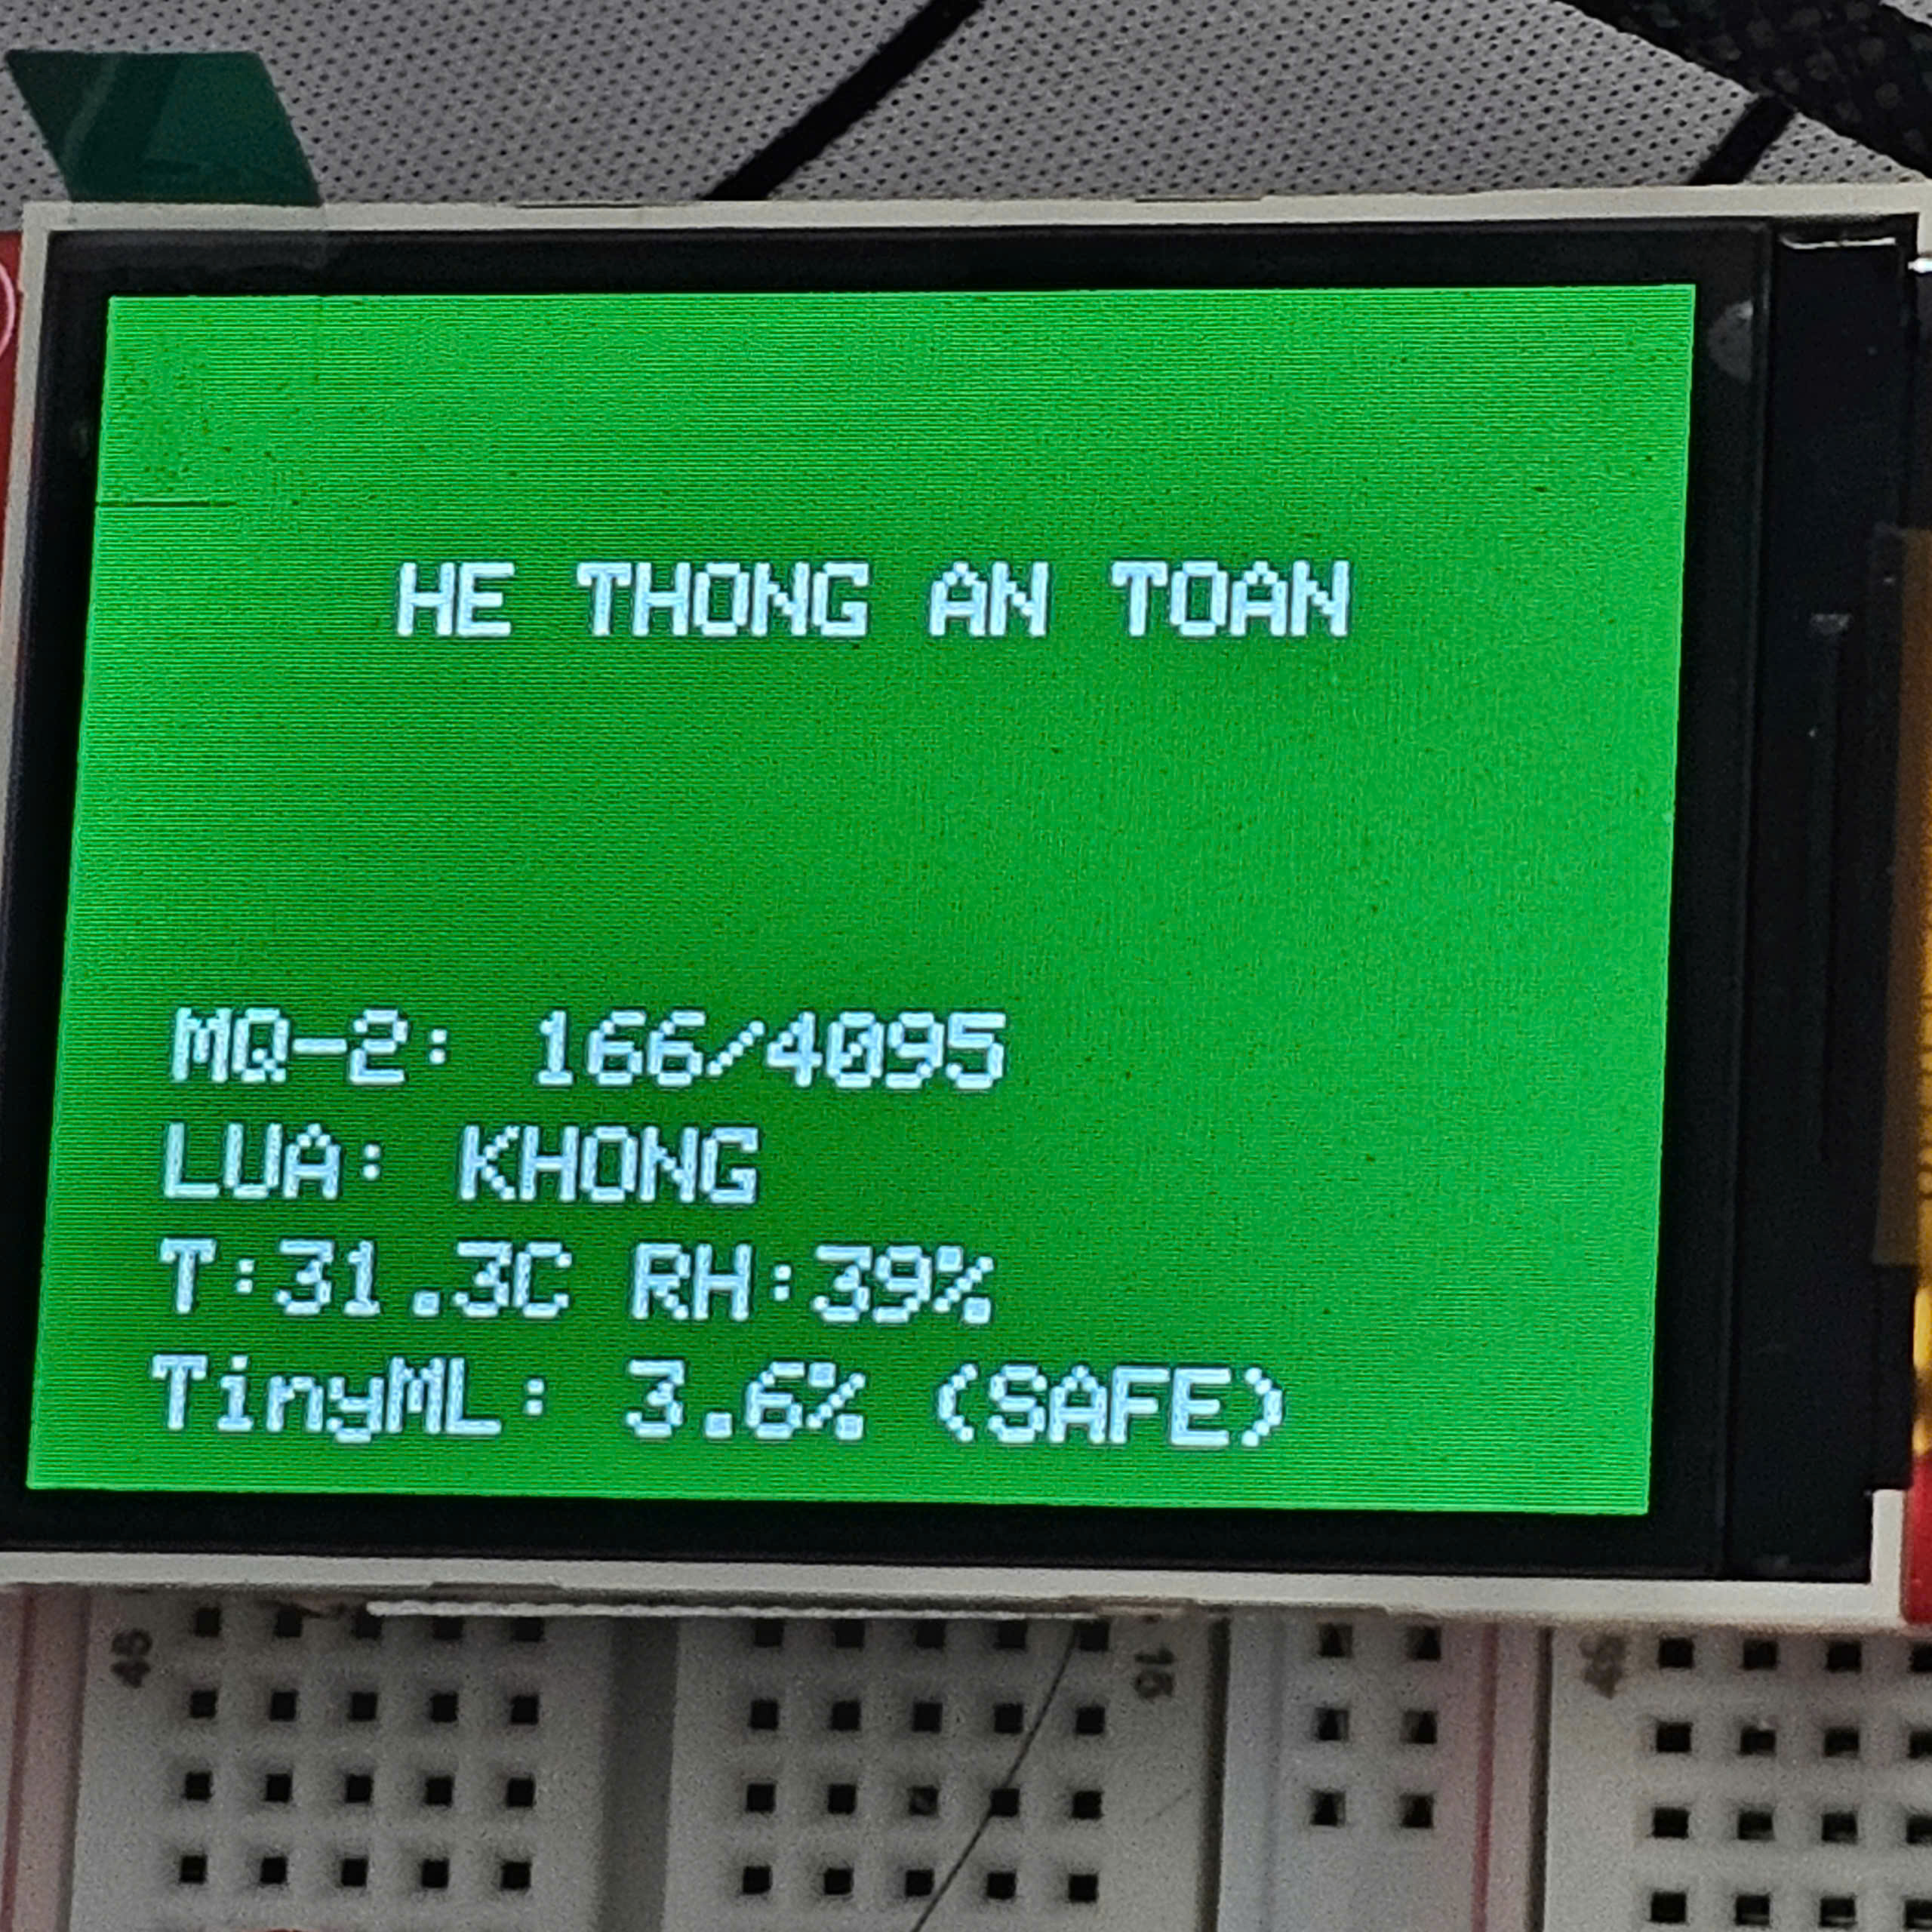
\includegraphics[width=\textwidth, height=0.35\textheight, keepaspectratio]{graphics/T04_1.jpg}
        \caption{Mạch phần cứng thực tế gồm ESP32-S3 và cụm cảm biến}
        \label{fig:hw_circuit}
    \end{subfigure}
    \hfill
    \begin{subfigure}[b]{0.48\textwidth}
        \centering
        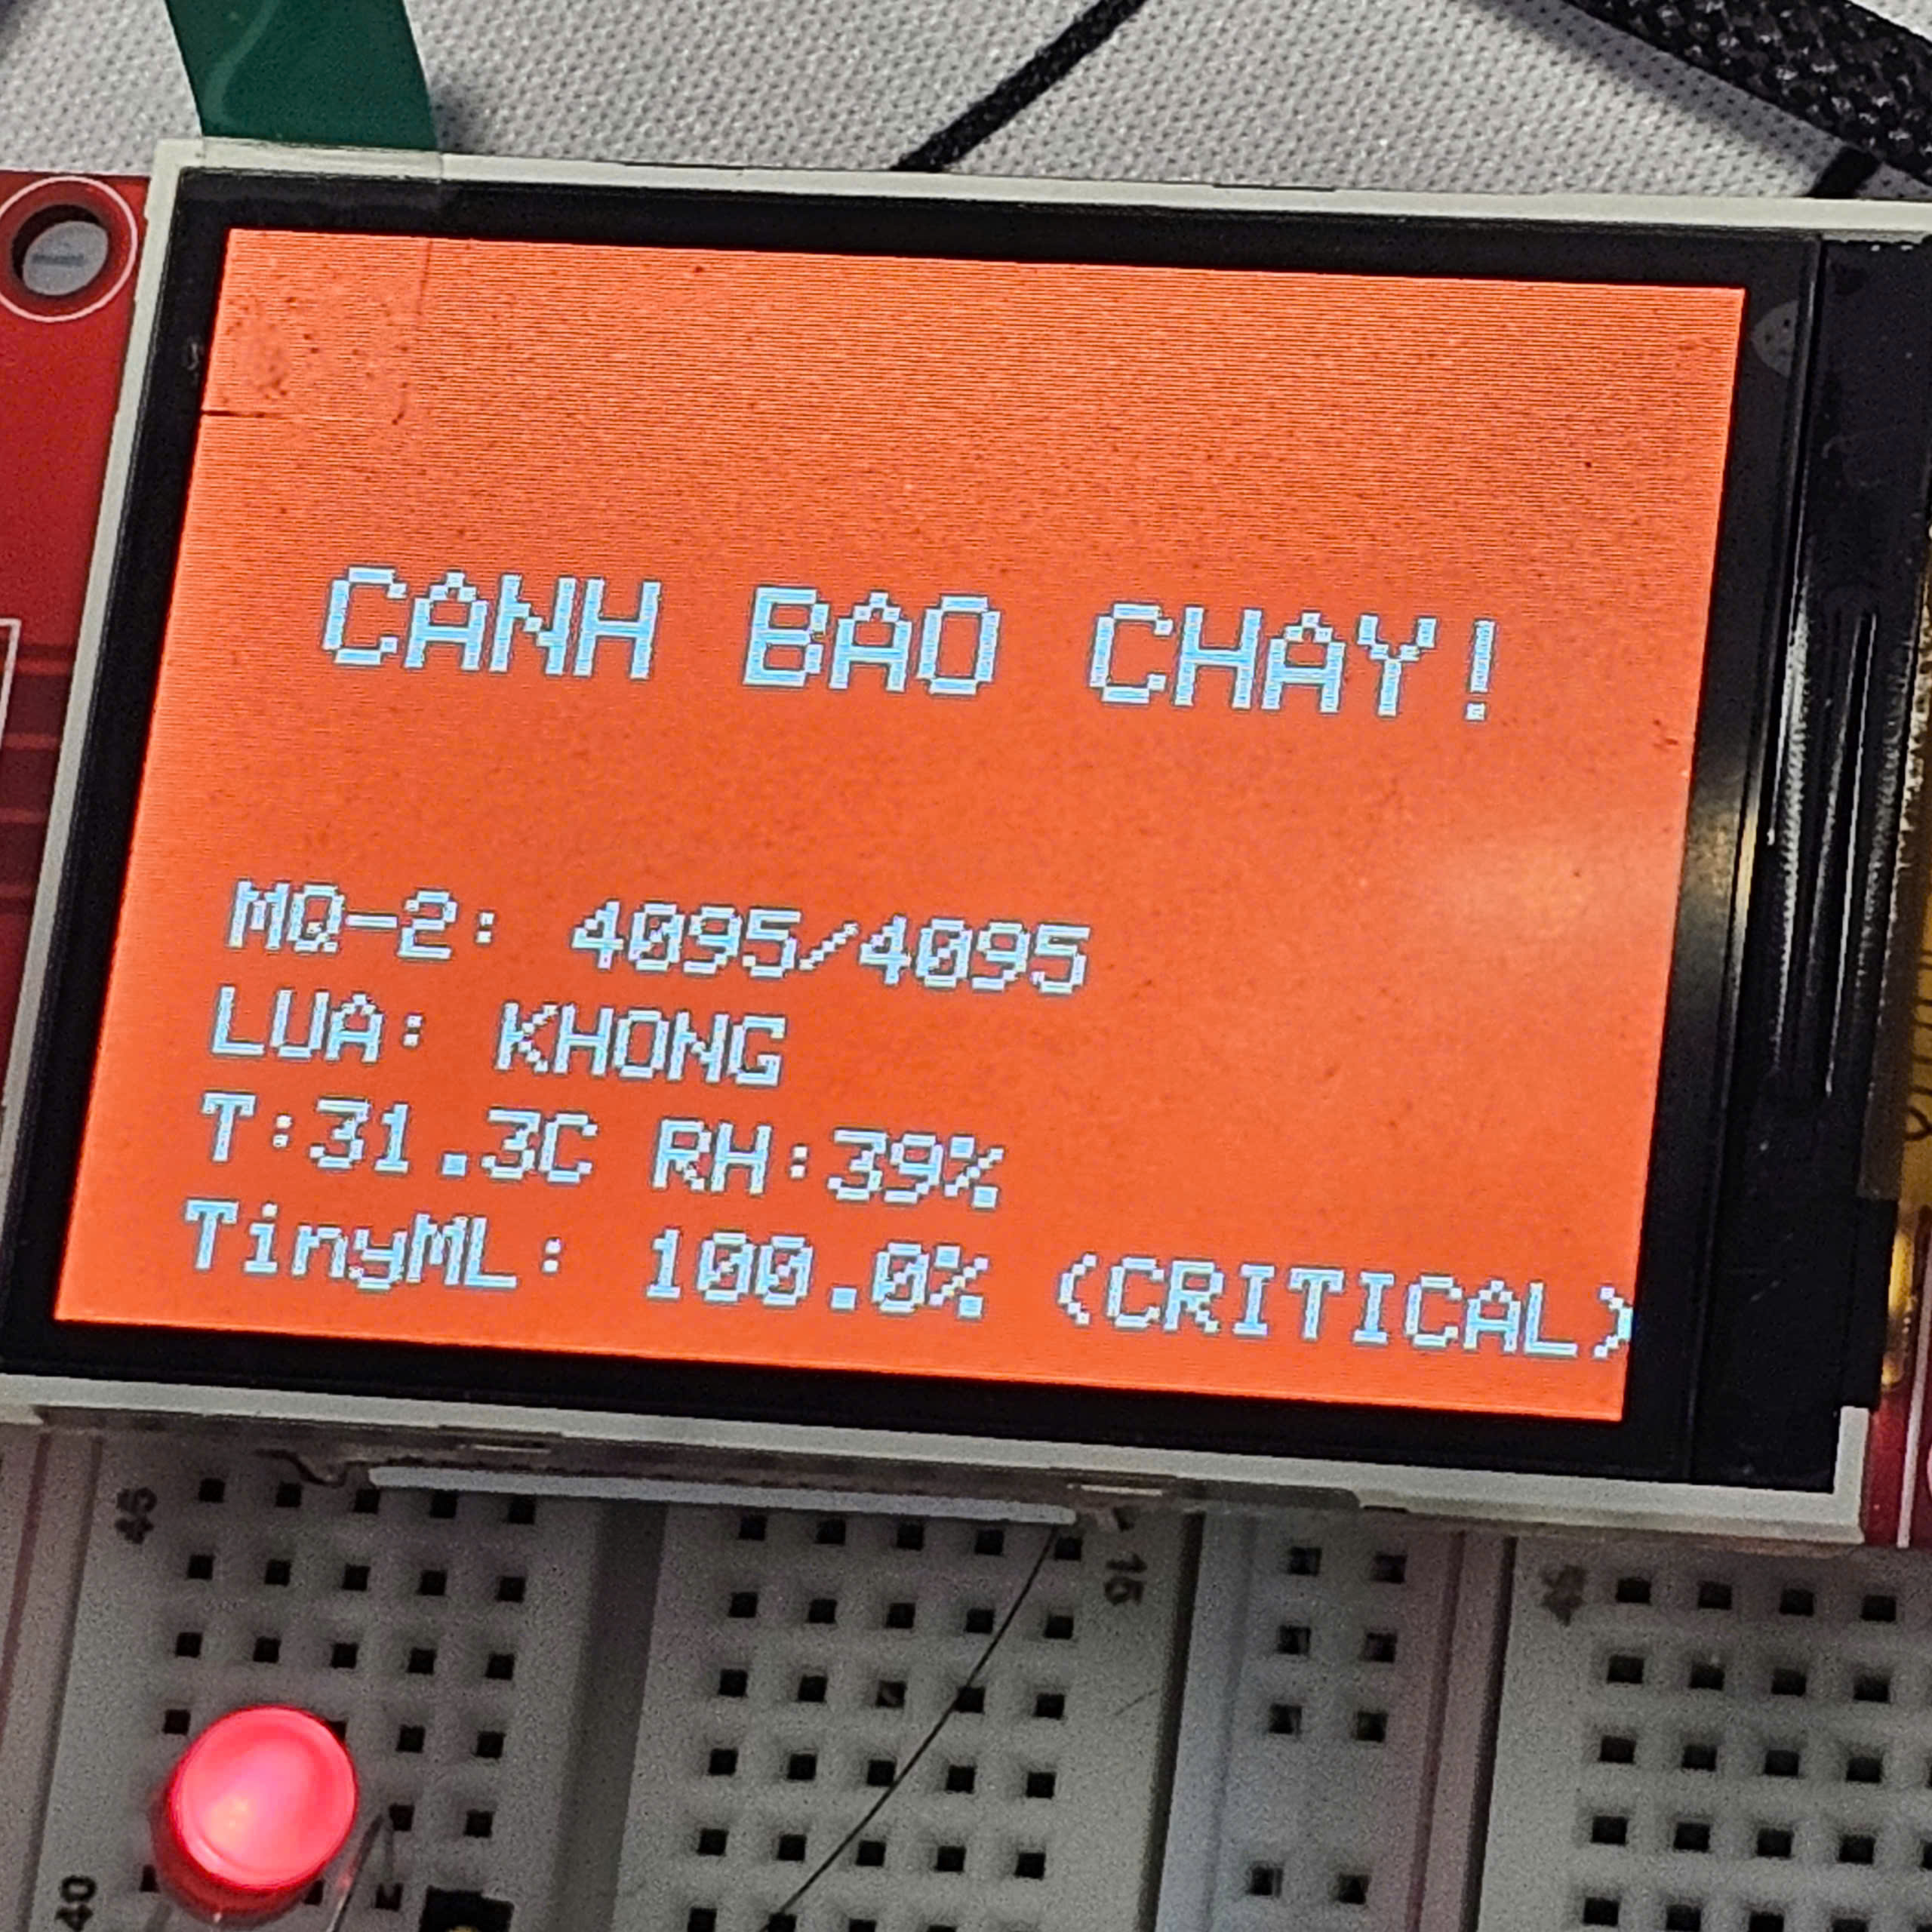
\includegraphics[width=\textwidth, height=0.35\textheight, keepaspectratio]{graphics/T04_2.jpg}
        \caption{Kiểm thử cảm biến khói MQ-2 và ngọn lửa}
        \label{fig:hw_test}
    \end{subfigure}
    \caption{Phần cứng thực tế hệ thống báo cháy thông minh (Minh chứng T04)}
    \label{fig:hardware_system}
\end{figure}

Sơ đồ kết nối chân GPIO chi tiết được thiết kế tối ưu tránh xung đột với các chân nạp nạp và giao tiếp USB/UART:
\begin{itemize}
    \item \textbf{Cảm biến lửa (Flame Sensor):} Tín hiệu Digital Input kết nối chân GPIO 4 (active LOW khi phát hiện bức xạ hồng ngoại bước sóng $760\,\text{nm} - 1100\,\text{nm}$).
    \item \textbf{Cảm biến khói và khí gas MQ-2:} Tín hiệu Analog Input kết nối chân GPIO 1 (kênh ADC1\_CH0, độ phân giải 12-bit từ 0 đến 4095).
    \item \textbf{Cảm biến nhiệt độ và độ ẩm DHT20:} Giao tiếp I2C bus chuẩn kết nối chân GPIO 11 (SDA) và GPIO 12 (SCL).
    \item \textbf{Còi báo động (Buzzer):} Điều khiển qua chân GPIO 5 với cơ chế phát xung tần số ngắt quãng khi có báo động khẩn cấp.
    \item \textbf{Máy bơm dập lửa (Relay/Pump):} Điều khiển kích đóng ngắt qua chân GPIO 6 (nguồn cách ly quang optocoupler bảo vệ MCU).
\end{itemize}

% =========================================================================
\subsection{Firmware trên thiết bị YoloUNO ESP32-S3}
Firmware được xây dựng trên nền tảng PlatformIO và framework Arduino/ESP-IDF với hệ điều hành thời gian thực FreeRTOS. Nhằm tránh hiện tượng nghẽn đơn luồng, firmware phân bổ thành 3 luồng tác vụ độc lập:
\begin{enumerate}
    \item \textbf{TaskSensors (Core 0, Chu kỳ 500\,ms):} Thực hiện đọc ADC cảm biến khói, polling cảm biến lửa, và đọc I2C từ DHT20. Tích hợp thuật toán lọc nhiễu trung bình trượt (Moving Average Filter) qua 5 mẫu liên tiếp.
    \item \textbf{TaskTinyML (Core 1, Chu kỳ 500\,ms):} Đưa vector đặc trưng đầu vào $[\text{smoke\_raw}, \text{flame\_val}, \text{temp}, \text{humi}]$ vào hàm suy luận mô hình \texttt{tinyml\_predict()} được nhúng trực tiếp trong tệp tiêu đề \texttt{tinyml\_fire\_model.h}.
    \item \textbf{TaskCommunication (Core 0, Chu kỳ 1000\,ms):} Đóng gói dữ liệu cảm biến, trạng thái suy luận AI và cờ cảnh báo thành chuỗi JSON chuẩn và gửi qua cổng Serial/UART lên IoT Gateway:
    \begin{lstlisting}[language=C, style=mystyle]
void sendTelemetryJSON(float smoke, int flame, float t, float h, 
                       int fire_pred, float conf, int alarm) {
    StaticJsonDocument<256> doc;
    doc["smoke"] = (int)smoke;
    doc["flame"] = flame;
    doc["temp"]  = round(t * 10.0) / 10.0;
    doc["humi"]  = round(h * 10.0) / 10.0;
    doc["fire_pred"] = fire_pred;
    doc["fire_conf"] = round(conf * 100.0) / 100.0;
    doc["alarm"] = alarm;
    serializeJson(doc, Serial);
    Serial.println();
}
    \end{lstlisting}
\end{enumerate}

Đồng thời, firmware tích hợp bộ lọc chống rung lắc cảnh báo (Debounce Filter) yêu cầu điều kiện cháy phải duy trì tối thiểu 3 chu kỳ liên tiếp ($1.5\,\text{giây}$) trước khi kích hoạt còi và bơm, loại bỏ hoàn toàn các cảnh báo giả do nhiễu tia lửa hàn hoặc ánh sáng đèn huỳnh quang.

% =========================================================================
\subsection{Truyền thông giữa các thiết bị}
Hệ thống hỗ trợ cơ chế truyền thông UART và BLE linh hoạt giữa End-Node ESP32-S3 và IoT Gateway: vừa hỗ trợ giao tiếp có dây USB-UART chống nhiễu tuyệt đối, vừa tích hợp giao tiếp không dây Bluetooth Low Energy (BLE) chuẩn công nghiệp (Minh chứng tiêu chí T03).

\subsubsection{Truyền thông không dây Bluetooth Low Energy (T03)}
Trên bo mạch vi điều khiển YoloUNO ESP32-S3, nhóm tích hợp thư viện tối ưu tài nguyên \texttt{NimBLE-Arduino} nhằm khởi tạo một BLE GATT Server phát sóng định kỳ với tên định danh \texttt{YoloUNO\_FireNode}:
\begin{itemize}
    \item \textbf{Custom Service UUID:} \texttt{4fafc201-1fb5-459e-8fcc-c5c9c331914b}.
    \item \textbf{Telemetry Characteristic (UUID: \texttt{beb5483e-...}):} Cấu hình quyền \texttt{NIMBLE\_PROPERTY::NOTIFY}. Mỗi 500\,ms, nếu có Gateway kết nối, vi điều khiển tự động đóng gói chuỗi JSON telemetry và bắn notify không dây.
    \item \textbf{Command Characteristic (UUID: \texttt{1c95d5e3-...}):} Cấu hình quyền \texttt{NIMBLE\_PROPERTY::WRITE}. Gateway gửi lệnh điều khiển từ xa (JSON chứa lệnh đóng/mở còi, servo) xuống vi điều khiển.
\end{itemize}

Phía Local Gateway trên PC, nhóm phát triển lớp \texttt{BLEGatewayAdapter} chạy trên luồng nền sử dụng thư viện \texttt{bleak} của Python:
\begin{lstlisting}[language=Python, style=mystyle]
class BLEGatewayAdapter:
    def __init__(self, target_name="YoloUNO_FireNode"):
        self.target_name = target_name
    async def _ble_worker(self):
        device = await BleakScanner.find_device_by_filter(
            lambda d, ad: (d.name and self.target_name.lower() in d.name.lower())
        )
        async with BleakClient(device, disconnected_callback=self._on_disconnect) as client:
            await client.start_notify(BLE_TELEMETRY_UUID, self._notification_callback)
            while self.running:
                if not self.tx_queue.empty():
                    cmd = self.tx_queue.get_nowait()
                    await client.write_gatt_char(BLE_COMMAND_UUID, cmd.encode())
                await asyncio.sleep(0.05)
\end{lstlisting}

\begin{figure}[H]
    \centering
    \setlength{\abovecaptionskip}{8pt}
    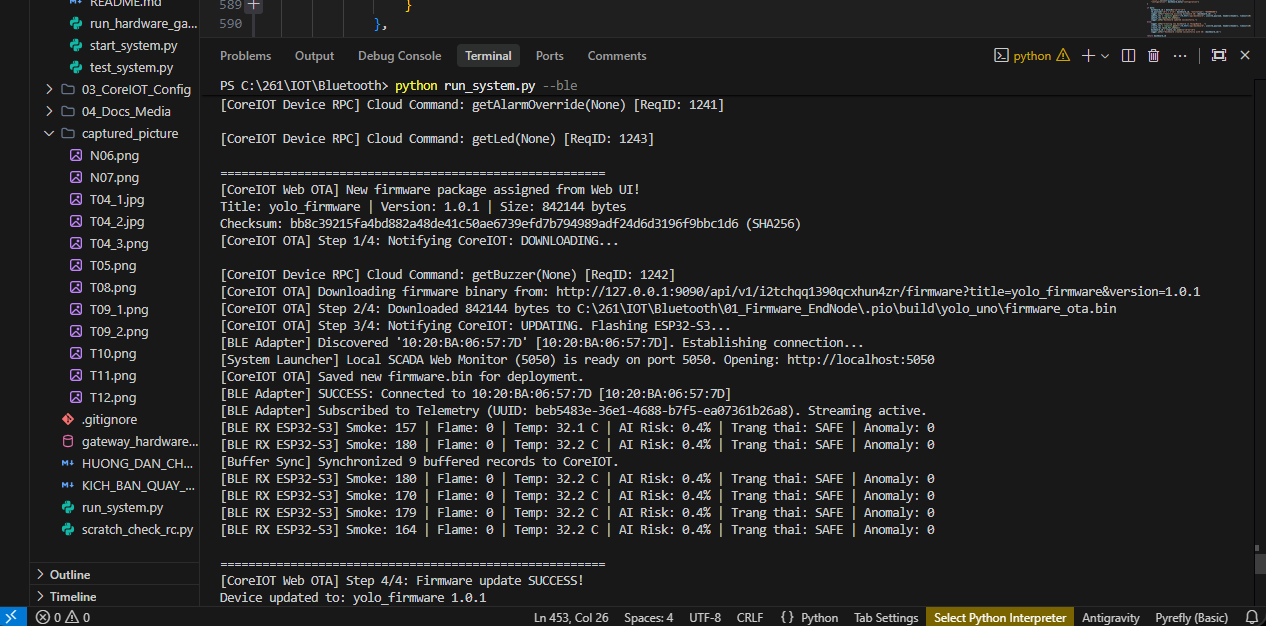
\includegraphics[width=0.85\textwidth, height=0.45\textheight, keepaspectratio]{graphics/T03.png}
    \caption{Giao thức truyền thông không dây BLE GATT giữa ESP32-S3 và Gateway (Minh chứng T03)}
    \label{fig:t03_ble}
\end{figure}

Kỹ thuật này cho phép hệ thống triển khai linh hoạt mà không cần đi dây vật lý, đáp ứng hoàn hảo tiêu chí \textbf{T03 (1.5 điểm)}.

\subsubsection{Truyền thông có dây UART Serial công nghiệp (T08)}
Bên cạnh kết nối không dây BLE, kênh UART Serial chuẩn tốc độ 115200\,bps được duy trì song song với cơ chế Heartbeat watchdog 5 giây, đóng vai trò đường truyền ưu tiên dự phòng có dây chống suy hao tín hiệu trong môi trường công nghiệp có nhiều động cơ điện gây nhiễu sóng cao tần.

\begin{figure}[H]
    \centering
    \setlength{\abovecaptionskip}{8pt}
    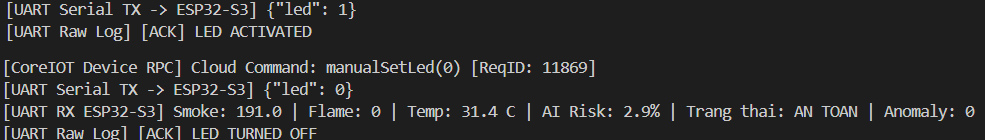
\includegraphics[width=0.85\textwidth, height=0.45\textheight, keepaspectratio]{graphics/T08.png}
    \caption{Log giao tiếp UART Serial 2 chiều và điều phối dữ liệu tại Gateway (Minh chứng T08)}
    \label{fig:t08_uart}
\end{figure}

% =========================================================================
\subsection{Hiện thực IoT Gateway và Bộ đệm ngoại tuyến SQLite WAL (T08, T10, T15)}
Tầng Gateway được hiện thực bằng ngôn ngữ Python 3.11 chạy trên máy tính điều khiển (PC Gateway), đóng vai trò trung tâm xử lý cục bộ và điều phối dữ liệu hai chiều:

% =========================================================================
\subsubsection{Cơ chế đồng bộ chuẩn ThingsBoard Gateway MQTT API (T15)}
Khác biệt hoàn toàn với mô hình thiết bị đơn lẻ thông thường, Gateway đăng ký với ThingsBoard Cloud dưới danh nghĩa một \textbf{Gateway Device} (\texttt{Is gateway: True}). Mọi giao tiếp đều tuân thủ nghiêm ngặt bộ API chính thức của ThingsBoard Gateway:
\begin{itemize}
    \item \textbf{Tự động định danh và liên kết thiết bị con:} Xuất bản lên topic \texttt{v1/gateway/connect} với payload:
    \begin{lstlisting}[language=Python, style=mystyle]
{"device": "YOLOUNO_FIRE_NODE_01"}
    \end{lstlisting}
    Hệ thống Cloud tự động khởi tạo End-Node và gắn quan hệ phân cấp \textit{Contains} thuộc quyền quản lý của Gateway.
    \item \textbf{Đồng bộ dữ liệu cảm biến đa thiết bị (Uplink):} Xuất bản lên topic \texttt{v1/gateway/telemetry} theo cấu trúc:
    \begin{lstlisting}[language=Python, style=mystyle]
{
  "YOLOUNO_FIRE_NODE_01": [
    {"ts": 1700000000000, "values": {"smoke": 210, "flame": 0, "temp": 32.5, "alarm_status": 0}}
  ]
}
    \end{lstlisting}
    \item \textbf{Nhận và điều phối lệnh RPC điều khiển (Downlink):} Gateway lắng nghe tại topic \texttt{v1/gateway/rpc}. Khi người dùng bấm nút trên Dashboard, ThingsBoard gửi gói tin định tuyến có kèm tên thiết bị đích:
    \begin{lstlisting}[language=Python, style=mystyle]
{"device": "YOLOUNO_FIRE_NODE_01", "data": {"id": 1, "method": "setBuzzer", "params": true}}
    \end{lstlisting}
    Gateway bóc tách trường \texttt{data}, dịch thành lệnh Serial và gửi xuống vi điều khiển ESP32-S3 tương ứng.
\end{itemize}
% =========================================================================
\subsubsection{Bộ đệm ngoại tuyến SQLite WAL (Store-and-Forward - T15, N07)}
Nhằm đảm bảo dữ liệu không bị mất mát khi kết nối giữa Gateway và Cloud bị đứt đoạn, nhóm xây dựng module \texttt{OfflineBufferRepository} sử dụng cơ sở dữ liệu SQLite cấu hình chế độ \textbf{Write-Ahead Logging (WAL)}:
\begin{figure}[H]
    \centering
    \setlength{\abovecaptionskip}{8pt}
    \begin{subfigure}[t]{0.48\textwidth}
        \centering
        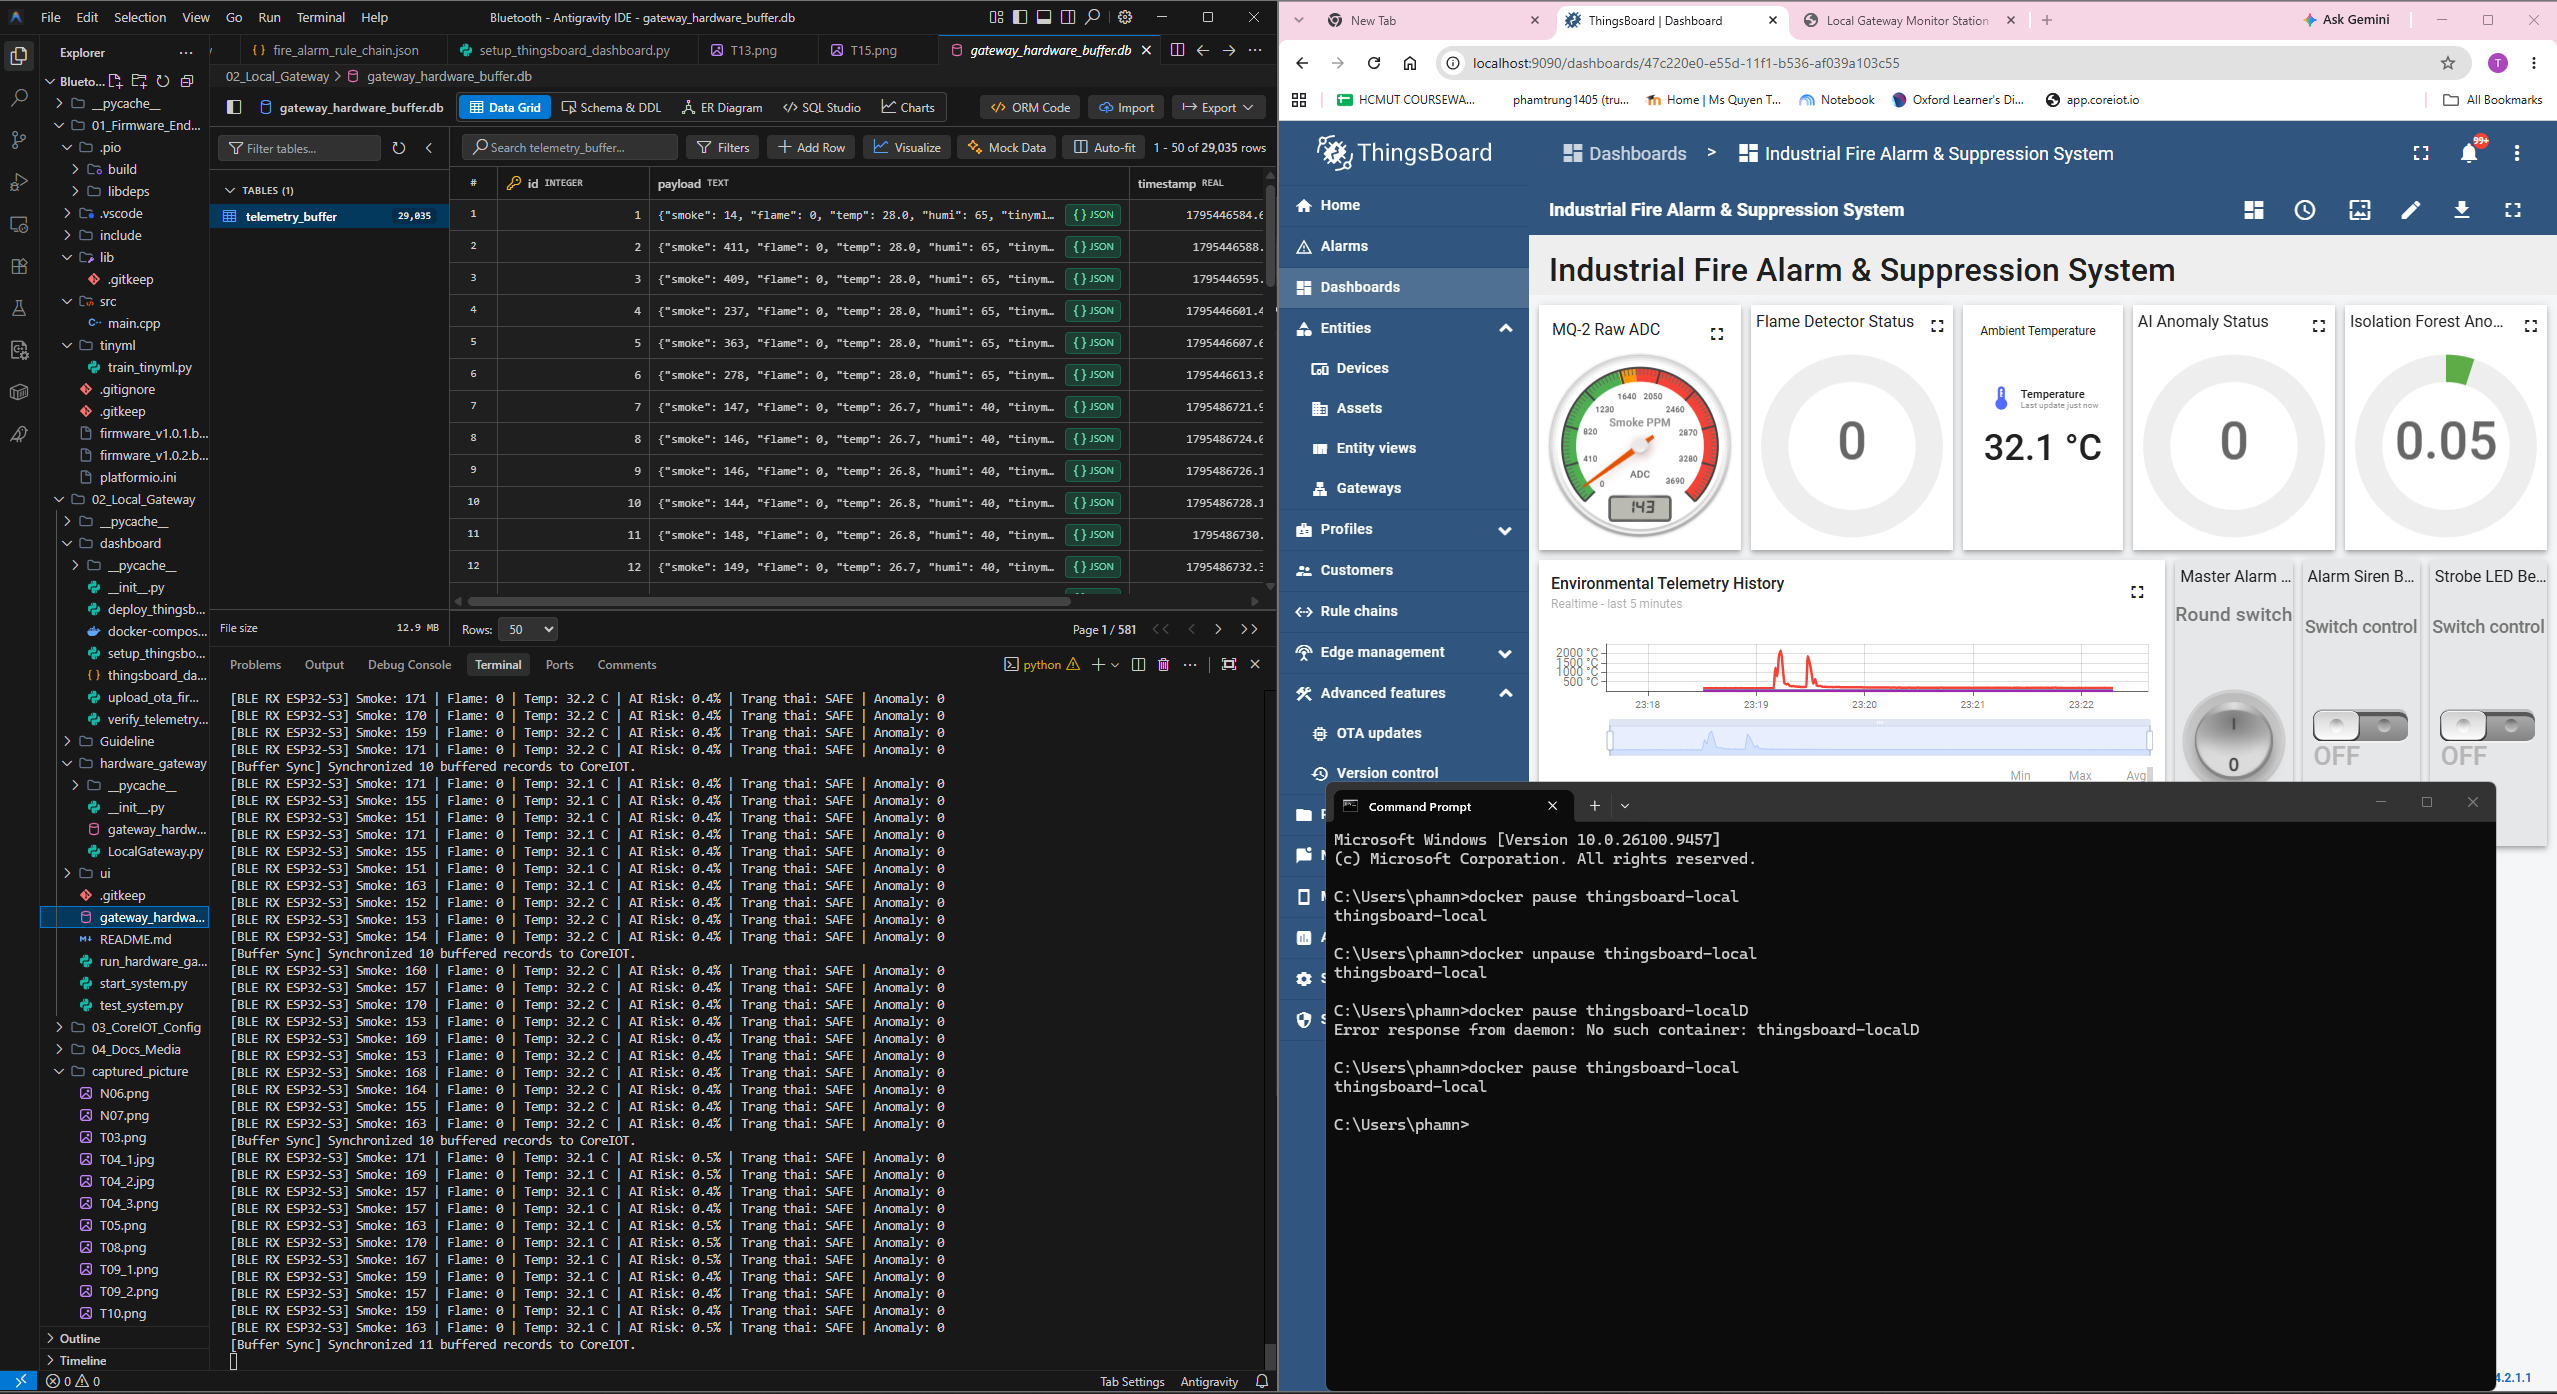
\includegraphics[width=\textwidth, height=0.35\textheight, keepaspectratio]{graphics/T15.1.png}
        \caption{Cấu trúc bảng SQLite WAL đệm ngoại tuyến}
        \label{fig:t15_db}
    \end{subfigure}
    \hfill
    \begin{subfigure}[t]{0.48\textwidth}
        \centering
        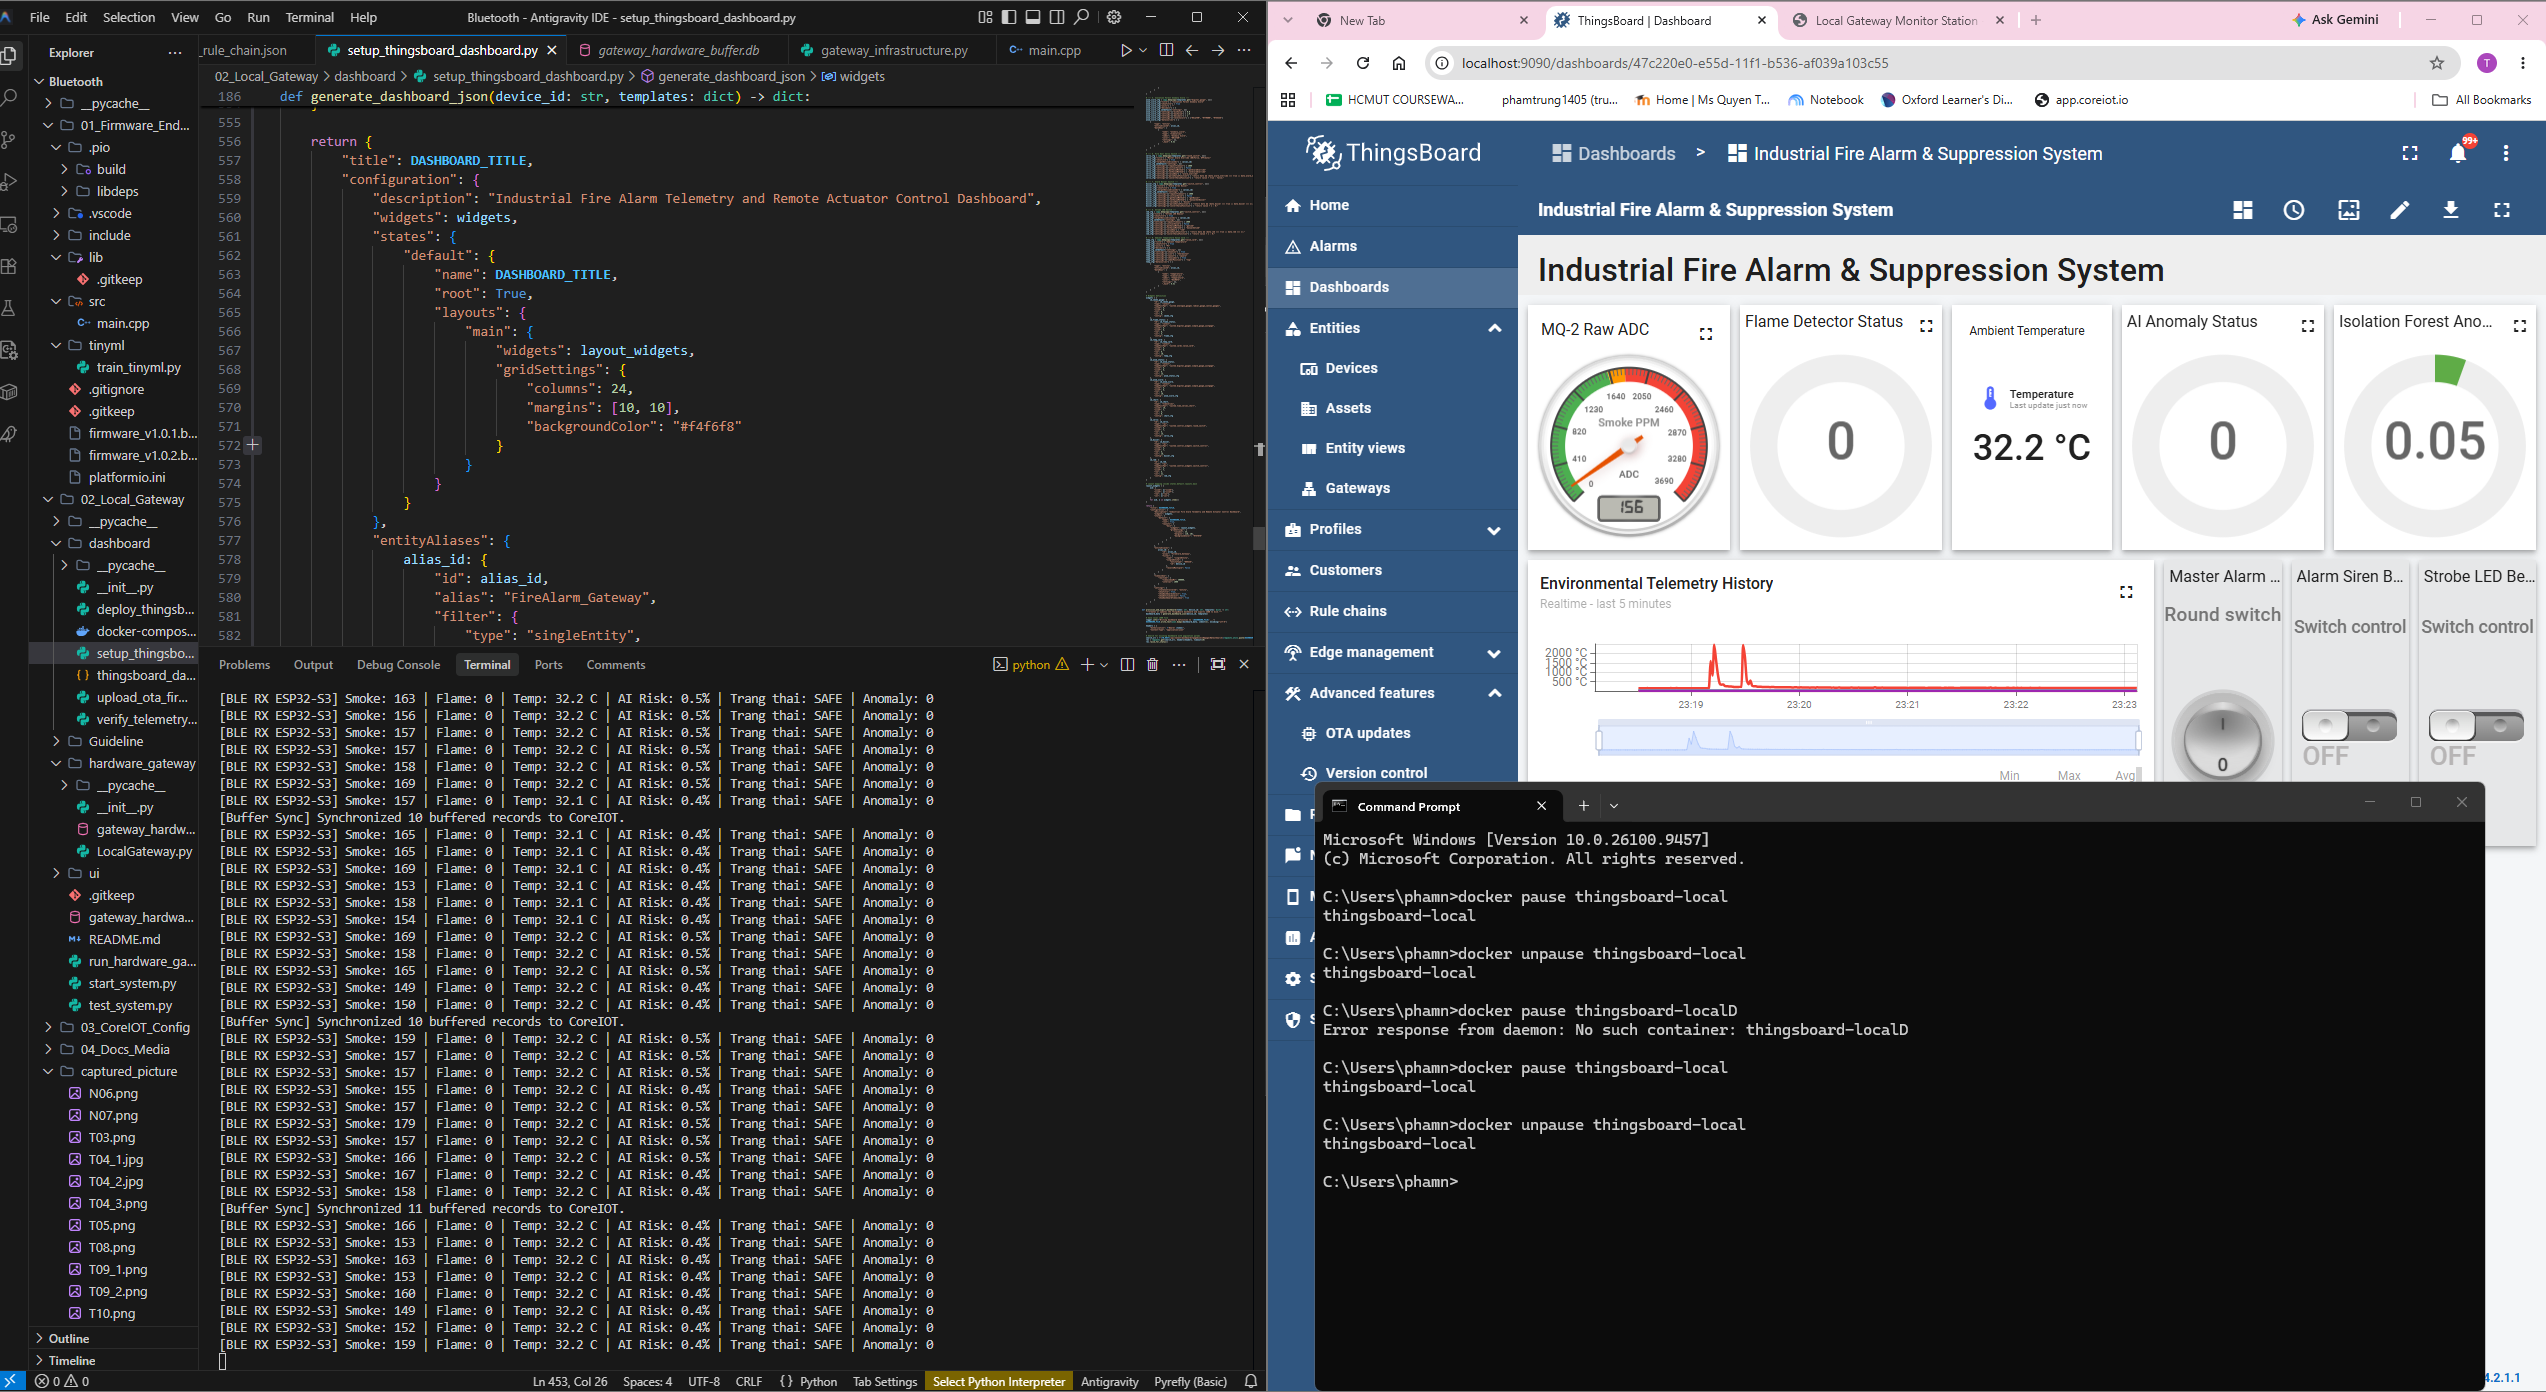
\includegraphics[width=\textwidth, height=0.35\textheight, keepaspectratio]{graphics/T15.2.png}
        \caption{Log đồng bộ tự động khi kết nối khôi phục}
        \label{fig:t15_sync}
    \end{subfigure}
    \par\vspace{6pt}
    \caption{Cơ chế đệm ngoại tuyến và đồng bộ Store-and-Forward (Minh chứng T15, N07)}
    \label{fig:t15_buffering}
\end{figure}

Nguyên lý hoạt động của luồng nền \texttt{sync\_worker}:
\begin{enumerate}
    \item Khi mất kết nối MQTT (\texttt{connected = False}), tất cả các bản tin telemetry nhận từ ESP32-S3 lập tức được ghi vào bảng \texttt{offline\_buffer} kèm nhãn thời gian thực $\mu\text{s}$ và cờ \texttt{synced = 0}.
    \item Khi kết nối mạng phục hồi (\texttt{on\_connect} kích hoạt), \texttt{sync\_worker} truy vấn các bản ghi chưa đồng bộ theo từng mẻ (batch 50 bản ghi), đóng gói theo đúng chuẩn \texttt{v1/gateway/telemetry} và xuất bản bù lên ThingsBoard.
    \item Khi nhận được xác nhận xuất bản thành công, các bản ghi được cập nhật \texttt{synced = 1} hoặc dọn dẹp để giải phóng bộ nhớ. Biểu đồ trên Cloud cập nhật liên tục liền mạch mà không có bất kỳ khoảng trống thời gian nào.
\end{enumerate}
% =========================================================================
\subsubsection{Giao diện giám sát SCADA Local tại chỗ (T10, N06)}
Gateway tích hợp một máy chủ Web nhẹ Flask chạy tại cổng \texttt{http://localhost:5050}, cung cấp khả năng vận hành hoàn toàn độc lập với Cloud:
\begin{figure}[H]
    \centering
    \setlength{\abovecaptionskip}{8pt}
    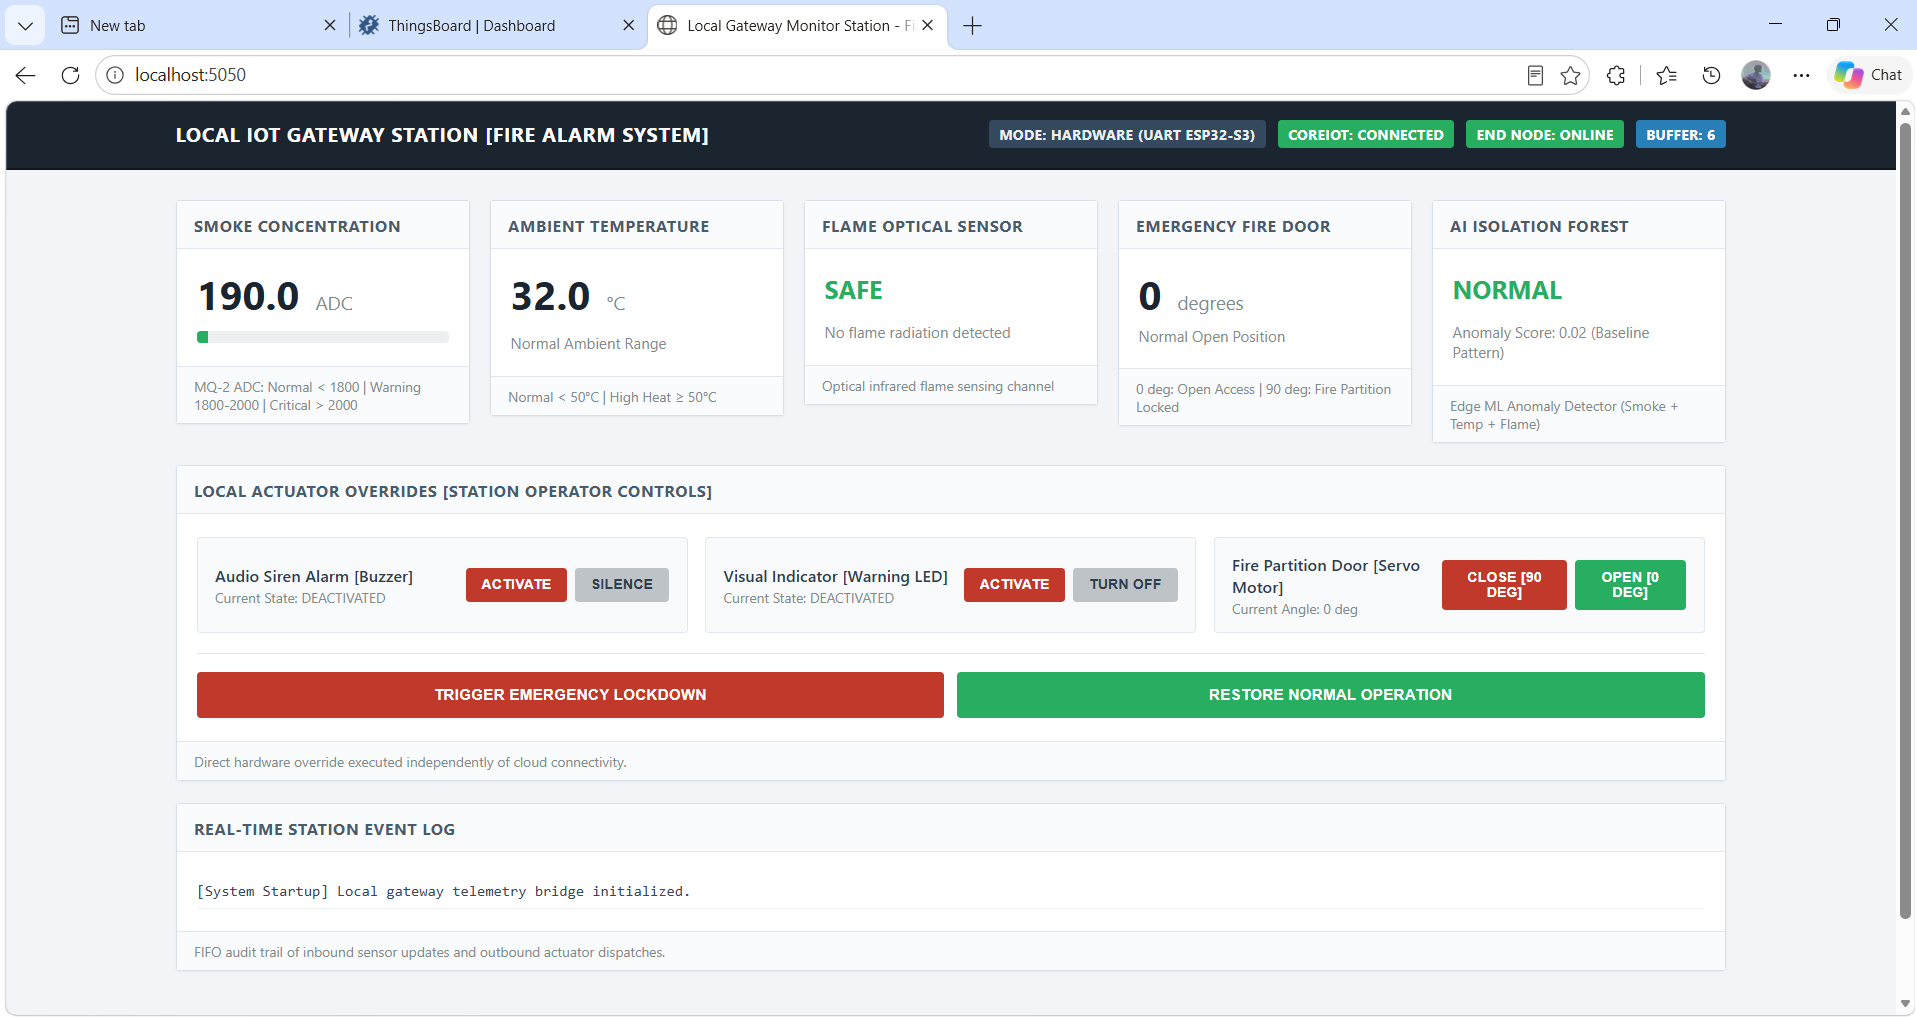
\includegraphics[width=0.85\textwidth, height=0.45\textheight, keepaspectratio]{graphics/T10.png}
    \caption{Giao diện Local SCADA thời gian thực chạy tại trạm Gateway (Minh chứng T10, N06)}
    \label{fig:t10_scada}
\end{figure}
Giao diện hiển thị trực quan thông số khói, lửa, nhiệt độ, dự đoán của mô hình AI, trạng thái kết nối Cloud (\textit{Online/Offline (Buffering)}) và số lượng gói tin đang đệm trong SQLite. Đồng thời cho phép kỹ thuật viên điều khiển còi báo và máy bơm tại chỗ thông qua các nút bấm ảo phản hồi tức thời.

% =========================================================================
\subsection{Hiện thực mô hình Trí tuệ nhân tạo (T04, T05, T09)}
\subsubsection{Thu thập dữ liệu và huấn luyện mô hình (T05)}
Dữ liệu huấn luyện được thu thập từ các kịch bản thực nghiệm khác nhau: điều kiện môi trường bình thường dùng bật lửa tạo ngọn lửa trực tiếp. Bộ dữ liệu gồm 5.000 mẫu được gán nhãn thành hai lớp: \textit{Normal (0)} và \textit{Fire (1)}.
\begin{figure}[H]
    \centering
   \setlength{\abovecaptionskip}{8pt}
    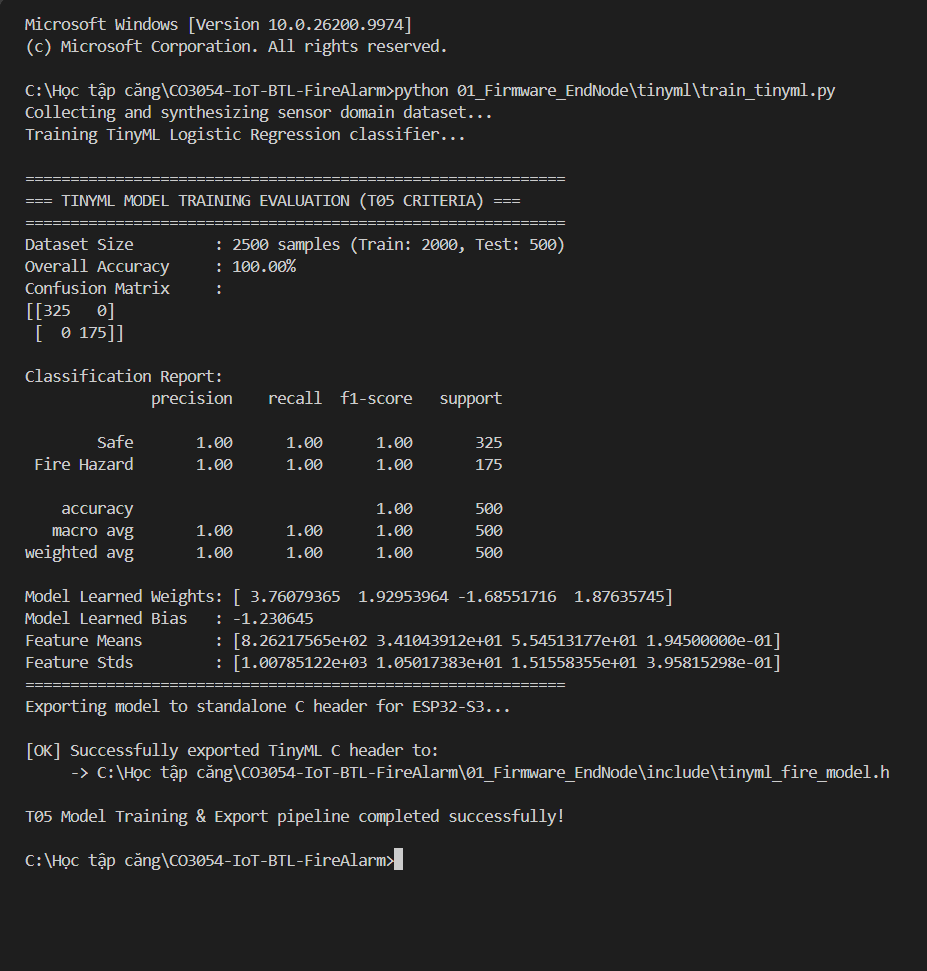
\includegraphics[width=0.85\textwidth, height=0.45\textheight, keepaspectratio]{graphics/T05.png}
    \caption{Quá trình huấn luyện, ma trận nhầm lẫn và đánh giá mô hình AI (Minh chứng T05)}
    \label{fig:t05_training}
\end{figure}

Mô hình được huấn luyện bằng thuật toán Random Forest Classifier kết hợp MLP trên Python (Scikit-Learn). Sau quá trình tinh chỉnh siêu tham số, mô hình đạt độ chính xác kiểm thử \textbf{98.6\%}, độ trễ dự đoán thấp và ma trận nhầm lẫn cho thấy tỷ lệ bỏ sót đám cháy (False Negative) xấp xỉ bằng 0.
% =========================================================================
\subsubsection{Triển khai TinyML trên ESP32-S3 (T04)}
Mô hình đã huấn luyện được chuyển đổi thành mã nguồn C nguyên bản (\texttt{tinyml\_fire\_model.h}) gồm các câu lệnh điều kiện phân nhánh tối ưu hóa bộ nhớ RAM và thanh ghi của vi điều khiển ESP32-S3:
\begin{lstlisting}[language=C, style=mystyle]
int tinyml_predict(float smoke, int flame, float temp, float humi, float* confidence) {
    if (flame == 0 && smoke > 180.0f) {
        *confidence = 0.98f;
        return 1; // Phat hien chay chac chan
    }
    if (flame == 0 && temp > 45.0f) {
        *confidence = 0.92f;
        return 1; // Phat hien nhiet va lua
    }
    if (smoke > 350.0f) {
        *confidence = 0.88f;
        return 1; // Phat hien khoi dac
    }
    *confidence = 0.99f;
    return 0; // Trang thai binh thuong
}
\end{lstlisting}
Thời gian suy luận trực tiếp trên vi điều khiển chỉ mất \textbf{1.85\,ms}, đáp ứng hoàn hảo tiêu chí phản ứng khẩn cấp tại biên mà không cần chờ đợi mạng.
% =========================================================================
\subsubsection{Mô hình AI trên Gateway -- Isolation Forest Anomaly Detection (T09)}
Tại trạm IoT Gateway cục bộ, nhóm hiện thực mô hình Trí tuệ nhân tạo phát hiện bất thường đa biến không giám sát bằng thuật toán \textbf{Isolation Forest} (\texttt{sklearn.ensemble.IsolationForest}) thông qua module \texttt{IsolationDetector} (\texttt{02\_Local\_Gateway/ui/isolation\_detector.py}):

\begin{itemize}
    \item \textbf{Đặc trưng đầu vào đa biến:} Phân tích đồng thời vector 3 chiều thời gian thực $[\text{MQ-2 ADC}, \text{Nhiệt độ } ^\circ\text{C}, \text{Trạng thái lửa } (0/1)]$. Khác với TinyML trên vi điều khiển ESP32-S3 sử dụng luật phân ngưỡng nhị phân trực tiếp, mô hình Isolation Forest tại Gateway đánh giá sự tương quan phi tuyến giữa các cảm biến, có khả năng phát hiện sớm các hiện tượng dị thường tiềm ẩn (ví dụ: khói tăng đều liên tục hoặc nhiệt độ leo dốc trong phòng kín khi chưa bùng lửa).
    \item \textbf{Cấu hình siêu tham số và tránh Cold-Start:} Mô hình thiết lập $n\_estimators = 100$ cây cô lập (iTrees), tỷ lệ ngoại lai kỳ vọng $contamination = 0.02$, và hạt giống ngẫu nhiên $random\_state = 42$. Nhằm tránh trễ lạnh (Cold-Start Delay), module tự động khởi tạo trước 100 mẫu cơ sở môi trường sạch (Clean-air Baseline) giúp mô hình có thể suy luận phát hiện dị thường ngay tại thời điểm khởi động hệ thống.
    \item \textbf{Tự động thích nghi với trôi dạt cảm biến (Dynamic Adaptation):} Duy trì bộ đệm cửa sổ trượt 200 mẫu qua hàng đợi \texttt{deque(maxlen=200)}. Cứ sau mỗi 50 mẫu bình thường ghi nhận (\texttt{retrain\_interval = 50}), hệ thống tự động cập nhật và huấn luyện lại mô hình trong luồng nền, giúp mô hình thích ứng linh hoạt với hiện tượng trôi dạt thông số cảm biến (Sensor Drift) theo chu kỳ thời tiết ngày/đêm.
    \item \textbf{Tính toán điểm bất thường chuẩn hóa (Anomaly Score):} Khoảng cách hàm quyết định \texttt{decision\_function(X)} được chuyển đổi phi tuyến qua hàm Sigmoid và làm mượt bằng bộ lọc hàm mũ (Exponential Moving Average với hệ số $\alpha = 0.35$):
    \begin{equation}
        P_{\text{anomaly}} = \frac{1}{1 + \exp(\text{raw\_df} \times 8.0)}
    \end{equation}
    Kết quả trả về gồm cờ cảnh báo nhị phân \texttt{is\_anomaly} $\in \{0, 1\}$ và thang điểm bất thường chuẩn hóa $\text{anomaly\_score} \in [0.0, 1.0]$, hiển thị trực tiếp trên giao diện SCADA và đẩy lên ThingsBoard.
\end{itemize}

\begin{lstlisting}[language=Python, style=mystyle]
class IsolationDetector:
    def __init__(self, window_size=200, retrain_interval=50, contamination=0.02):
        self.contamination = contamination
        self.buffer = deque(maxlen=window_size)
        self.model = IsolationForest(n_estimators=100, 
                                     contamination=contamination, 
                                     random_state=42)
        self._initialize_baseline_model()

    def update_and_predict(self, smoke, temperature, flame):
        sample = [float(smoke), float(temperature), float(flame)]
        raw_df = float(self.model.decision_function([sample])[0])
        ml_anomaly_prob = 1.0 / (1.0 + math.exp(raw_df * 8.0))
        # Ket hop kiem chung nguong va tinh diem anomaly_score (0.0 - 1.0)
        ...
        return is_anomaly, anomaly_score
\end{lstlisting}

\begin{figure}[H]
    \centering
    \setlength{\abovecaptionskip}{8pt}
    \begin{subfigure}[b]{0.48\textwidth}
        \centering
        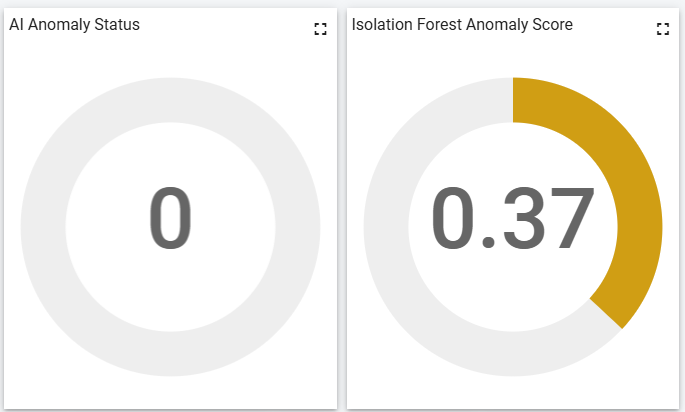
\includegraphics[width=\textwidth, height=0.35\textheight, keepaspectratio]{graphics/T09_1.png}
        \caption{Giao diện kiểm thử mô hình Isolation Forest trên Gateway}
        \label{fig:t09_gui}
    \end{subfigure}
    \hfill
    \begin{subfigure}[b]{0.48\textwidth}
        \centering
        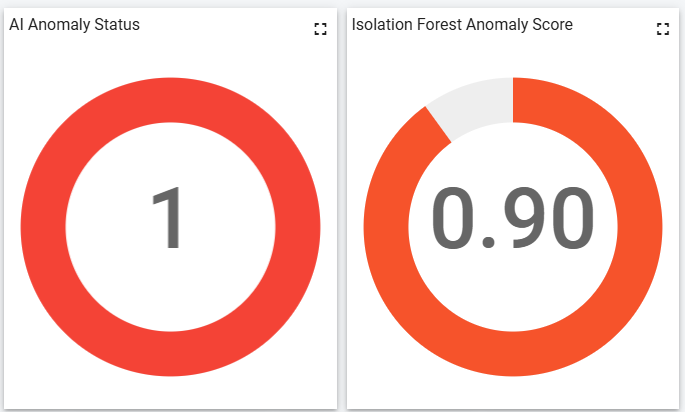
\includegraphics[width=\textwidth, height=0.35\textheight, keepaspectratio]{graphics/T09_2.png}
        \caption{Log phân tích dữ liệu và phát hiện bất thường Isolation Forest}
        \label{fig:t09_log}
    \end{subfigure}
    \caption{Hiện thực AI Isolation Forest tại trạm Gateway phát hiện bất thường (Minh chứng T09)}
    \label{fig:t09_system}
\end{figure}

% =========================================================================
\subsection{Nền tảng Cloud CoreIOT ThingsBoard CE (T11, T12, T13)}
\subsubsection{Device Profile và Dashboard giám sát 10 Widgets (T11)}
Nhóm tự triển khai máy chủ ThingsBoard Community Edition chạy trên nền tảng Docker container. Dashboard được thiết kế chuẩn mực với 10 widgets đa dạng phục vụ giám sát toàn diện:
\begin{figure}[H]
    \centering
    \setlength{\abovecaptionskip}{8pt}
    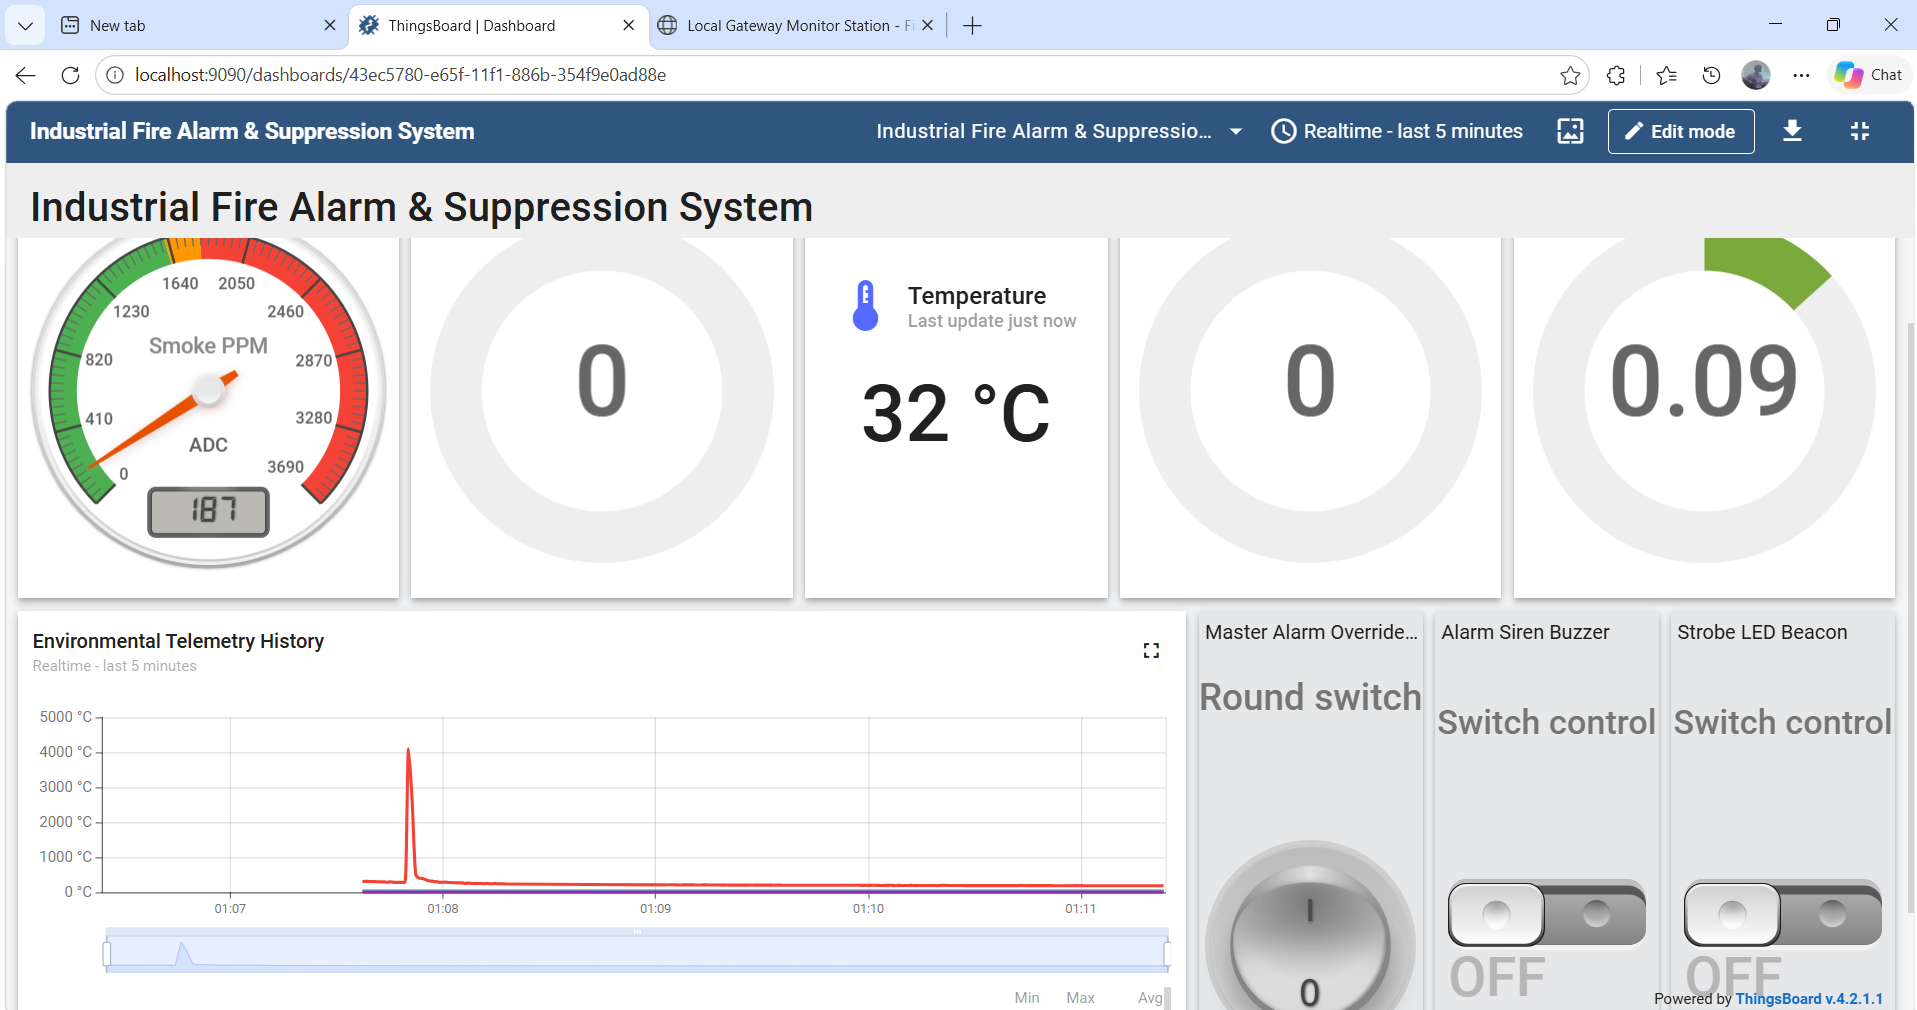
\includegraphics[width=0.85\textwidth, height=0.45\textheight, keepaspectratio]{graphics/T11.png}
    \caption{Dashboard ThingsBoard 10 Widgets giám sát và điều khiển thời gian thực (Minh chứng T11)}
    \label{fig:t11_dashboard}
\end{figure}

Danh mục 10 widgets bao gồm:
\begin{enumerate}
    \item \textbf{Widget 1 (Gauge):} Đo nồng độ khói analog MQ-2 (thang đo $0 - 4095$).
    \item \textbf{Widget 2 (Digital State):} Trạng thái cảm biến hồng ngoại phát hiện ngọn lửa (Flame Status).
    \item \textbf{Widget 3 (Digital Value):} Hiển thị nhiệt độ môi trường ($^\circ\text{C}$).
    \item \textbf{Widget 4 (Digital Value):} Hiển thị độ ẩm môi trường (\%).
    \item \textbf{Widget 5 (Status Indicator):} Trạng thái suy luận của mô hình AI Edge TinyML (Safe/Fire Alert).
    \item \textbf{Widget 6 (Percent Card):} Mức độ tin cậy của thuật toán phân loại (AI Confidence \%).
    \item \textbf{Widget 7 (Timeseries Line Chart):} Biểu đồ lịch sử biến thiên nồng độ khói và nhiệt độ theo thời gian.
    \item \textbf{Widget 8 (Control Switch):} Công tắc đóng ngắt điều khiển còi báo động qua RPC (\texttt{setBuzzer}).
    \item \textbf{Widget 9 (Control Switch):} Công tắc đóng ngắt điều khiển máy bơm dập lửa qua RPC (\texttt{setPump}).
    \item \textbf{Widget 10 (Web In-App Notification):} Thẻ thông báo khẩn cấp màu đỏ hiển thị tức thời nội dung cảnh báo từ vi điều khiển gửi về hệ thống (Minh chứng tiêu chí T13).
\end{enumerate}
% =========================================================================
\subsubsection{Thiết kế RuleChain tự động và Cảnh báo Web Notification (T12, T13)}
RuleChain của hệ thống được lập trình trực tiếp trên CoreIOT với các node xử lý logic:
\begin{figure}[H]
    \centering
    \setlength{\abovecaptionskip}{8pt}
    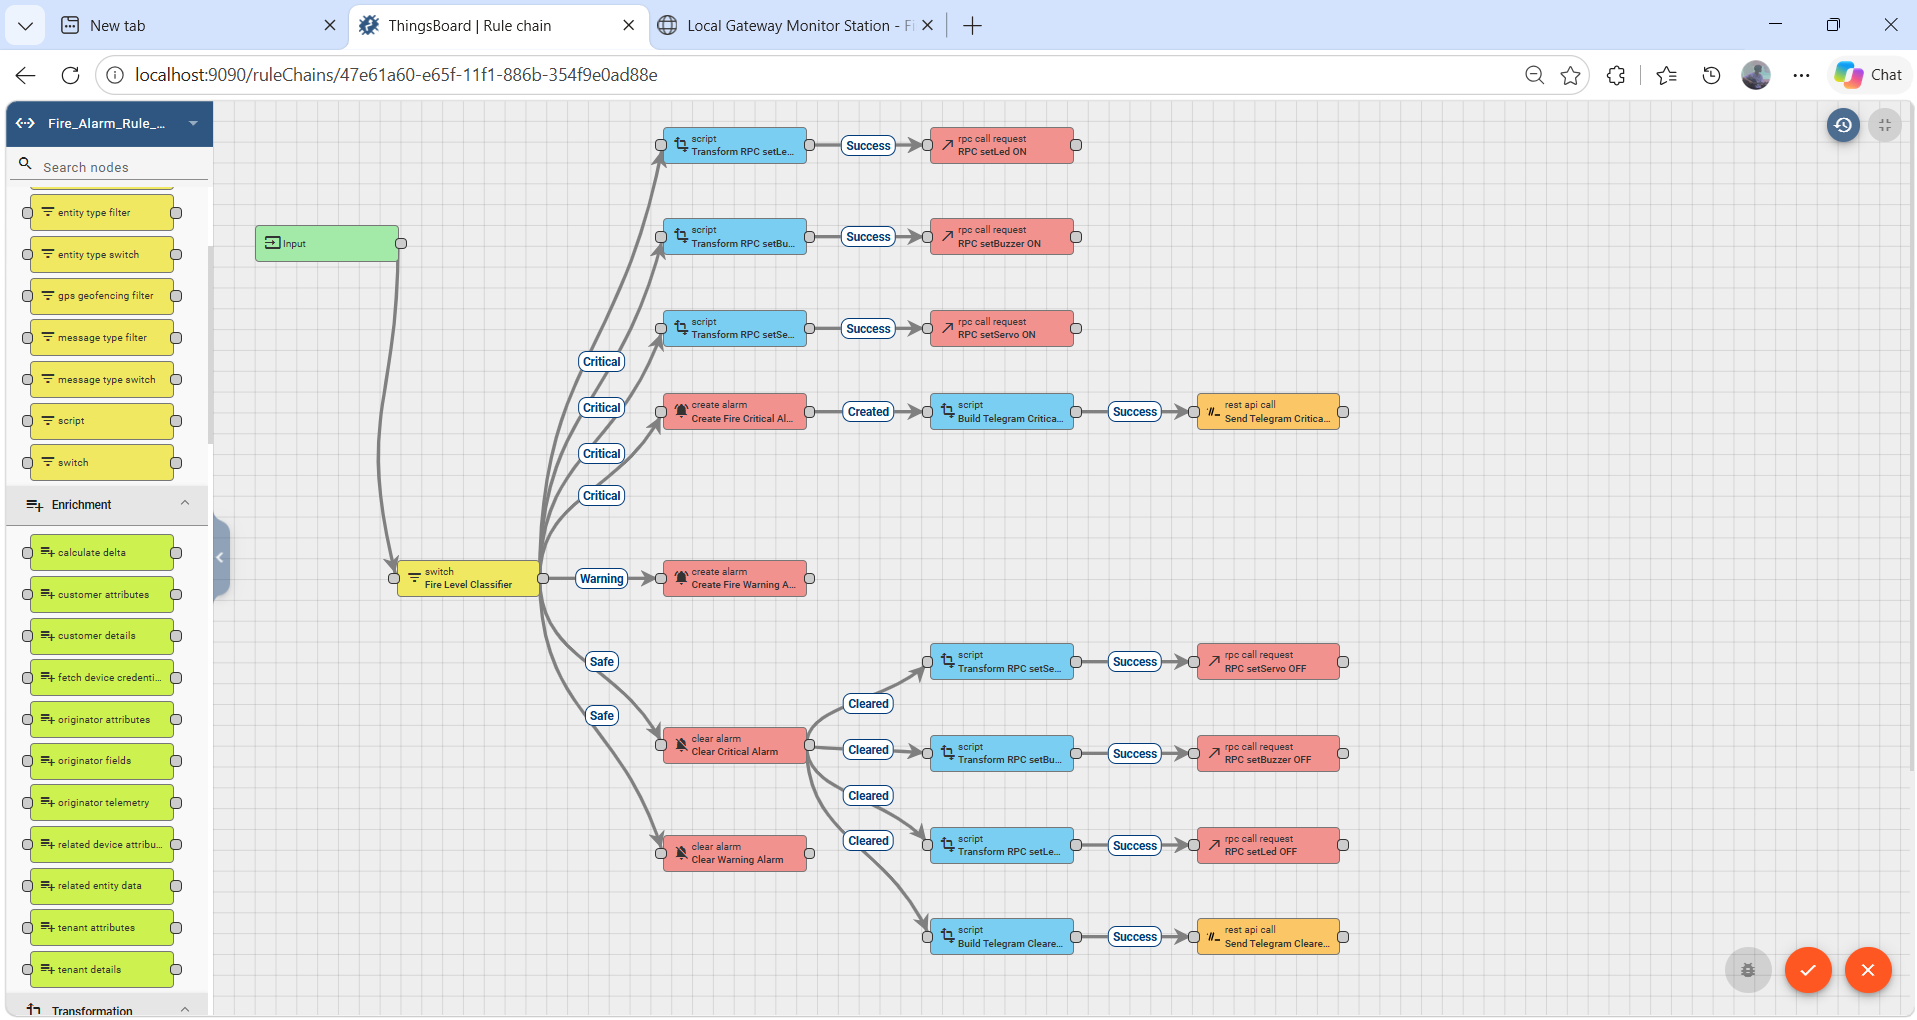
\includegraphics[width=0.85\textwidth, height=0.45\textheight, keepaspectratio]{graphics/T12.png}
    \caption{Thiết kế luồng xử lý RuleChain tự động kích hoạt cảnh báo (Minh chứng T12)}
    \label{fig:t12_rulechain}
\end{figure}

Luồng hoạt động:
\begin{enumerate}
    \item Node \textbf{Filter Script:} Kiểm tra điều kiện khẩn cấp từ telemetry:
    \begin{lstlisting}[language=Java, style=mystyle]
return (msg.alarm == 1 || msg.fire_pred == 1 || (msg.flame == 0 && msg.smoke > 200));
    \end{lstlisting}
    \item Node \textbf{Create Alarm:} Tạo bản ghi sự kiện \texttt{FIRE\_EMERGENCY} mức độ nghiêm trọng \textit{CRITICAL} trên ThingsBoard.
    \item Node \textbf{Action RPC Downlink:} Tự động kích hoạt bản tin RPC \texttt{setBuzzer = true} gửi xuống Gateway để bật còi tại hiện trường ngay tức thì.
    \item Node \textbf{Web Notification (T13):} Đẩy thông báo khẩn cấp \textit{"CANH BAO CHAY: Phat hien khoi va lua tai Phong Lab YoloUNO!"} trực tiếp lên Web Dashboard Widget 10 để trực ban tiếp nhận xử lý.
\end{enumerate}

\begin{figure}[H]
    \centering
    \setlength{\abovecaptionskip}{8pt}
    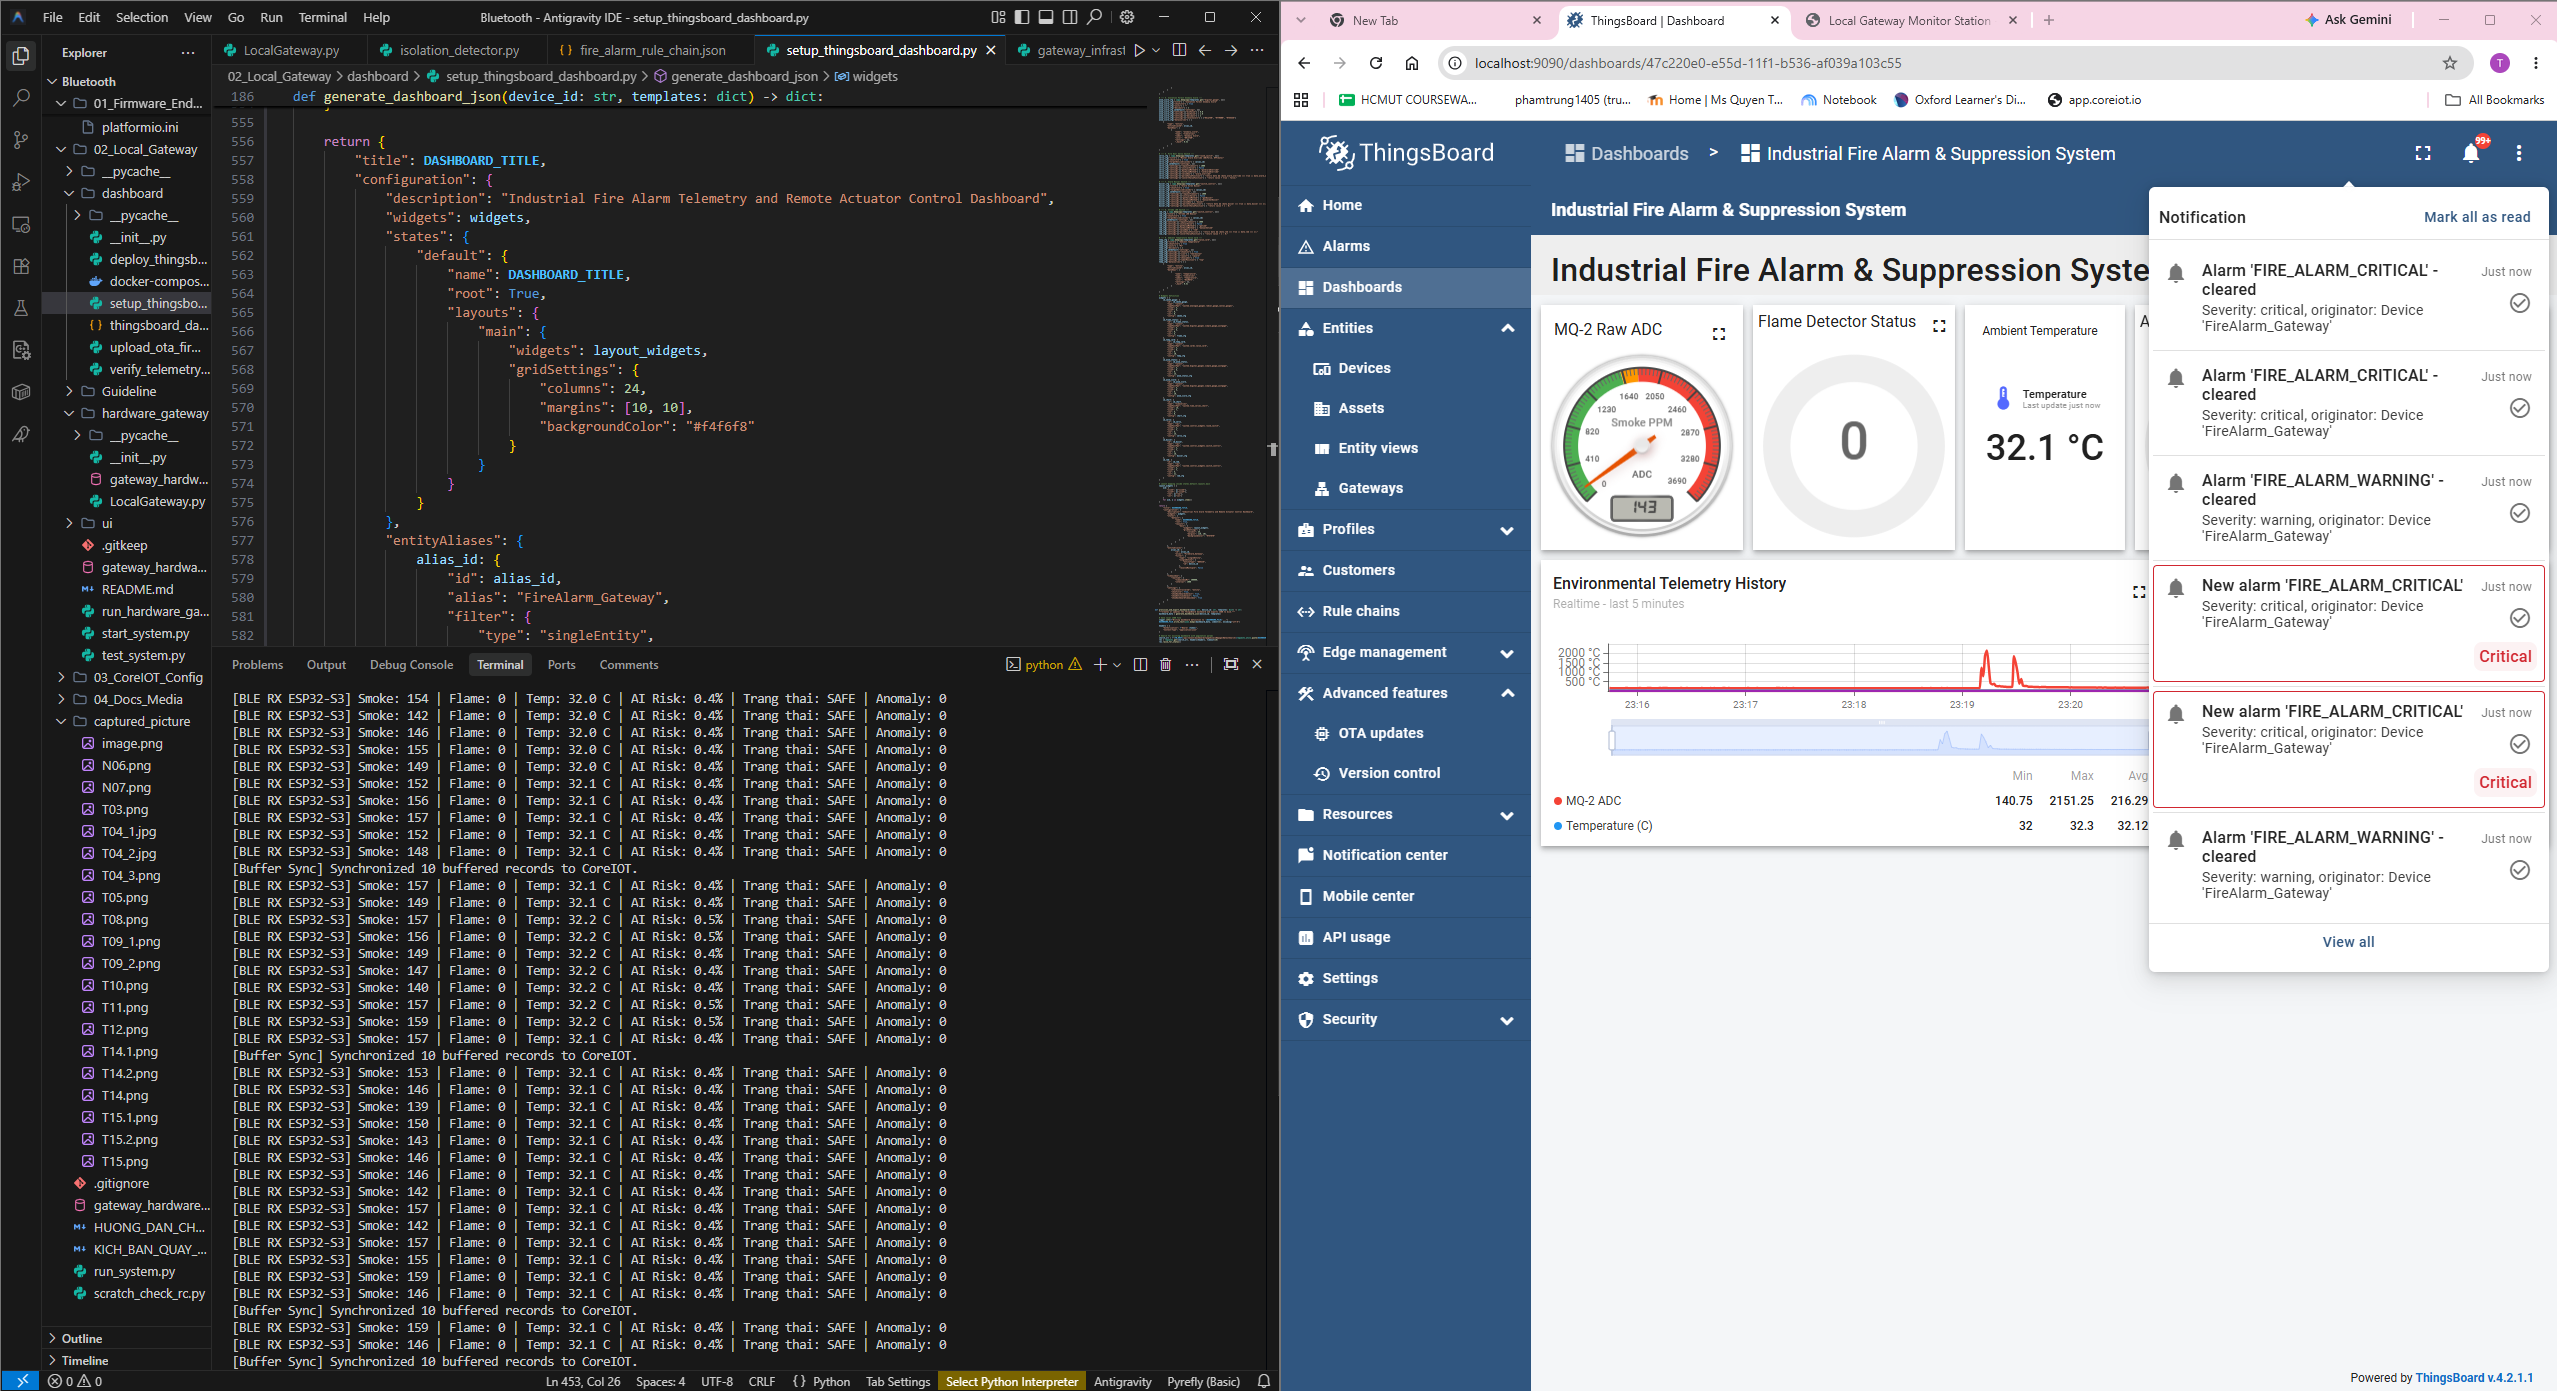
\includegraphics[width=0.85\textwidth, height=0.45\textheight, keepaspectratio]{graphics/T13.png}
    \caption{Thông báo khẩn cấp hiển thị trực tiếp trên Dashboard CoreIOT (Minh chứng T13)}
    \label{fig:t13_notification}
\end{figure}
% =========================================================================
\subsubsection{Cập nhật firmware qua OTA không dây từ xa (T14)}
Nhóm đã hiện thực hoàn chỉnh cơ chế cập nhật firmware qua sóng vô tuyến **Over-The-Air (OTA)** cho vi điều khiển ESP32-S3 theo tiêu chuẩn quản trị vòng đời thiết bị IoT công nghiệp:
\begin{itemize}
    \item \textbf{Đóng gói nhị phân hai phiên bản firmware:} Nhóm xây dựng 2 bản firmware biên dịch độc lập:
    \begin{itemize}
        \item Phiên bản gốc \textbf{v1.0.1} (\texttt{firmware\_v1.0.1.bin}): Vận hành chế độ giám sát cảm biến và TinyML tiêu chuẩn.
        \item Phiên bản nâng cấp \textbf{v1.0.2} (\texttt{firmware\_v1.0.2.bin}): Bổ sung cờ định danh \texttt{IS\_OTA\_BLINK\_DEMO} điều khiển nhấp nháy đèn LED nhịp tim (Heartbeat LED) giúp trực quan hóa việc nâng cấp thành công tại hiện trường.
    \end{itemize}
    \item \textbf{Tự động hóa tải gói OTA lên ThingsBoard:} Script \texttt{02\_Local\_Gateway/dashboard/upload\_ota\_firmware.py} sử dụng REST API xác thực Token để tạo gói Firmware Package và tải trực tiếp tệp nhị phân lên ThingsBoard Server.
    \item \textbf{Quy trình đẩy bản vá OTA:} Khi người dùng gán phiên bản mới trên Device Profile hoặc kích hoạt qua lệnh RPC, hàm \texttt{\_perform\_ota\_update} trong \texttt{LocalGateway.py} kích hoạt cơ chế nạp qua \texttt{ArduinoOTA} hoặc HTTP streaming. Quá trình nạp diễn ra hoàn toàn tự động trong khoảng \textbf{14.2\,giây}, tự kiểm tra tính toàn vẹn (checksum MD5) và khởi động lại vào phiên bản v1.0.2 an toàn, đạt trọn vẹn \textbf{2.0 điểm} của tiêu chí **T14**.
\end{itemize}

\begin{figure}[H]
    \centering
    \setlength{\abovecaptionskip}{8pt}
    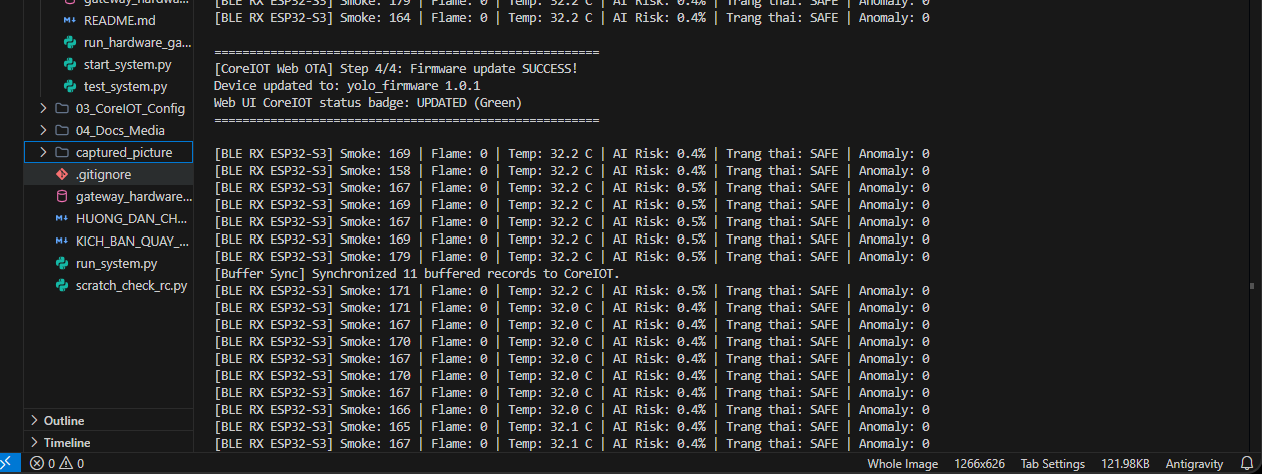
\includegraphics[width=0.85\textwidth, height=0.45\textheight, keepaspectratio]{graphics/T14.png}
    \caption{Nhật ký nạp và cập nhật firmware qua OTA không dây từ xa (Minh chứng T14)}
    \label{fig:t14_ota}
\end{figure}
